% ---------------------------------------------------------------------------
% Author guideline and sample document for EG publication using LaTeX2e input
% D.Fellner, v1.15, Dec 14, 2018

\documentclass{egpubl}
 
% --- for  Annual CONFERENCE
% \ConferenceSubmission   % uncomment for Conference submission
% \ConferencePaper        % uncomment for (final) Conference Paper
% \STAR                   % uncomment for STAR contribution
% \Tutorial               % uncomment for Tutorial contribution
% \ShortPresentation      % uncomment for (final) Short Conference Presentation
% \Areas                  % uncomment for Areas contribution
% \MedicalPrize           % uncomment for Medical Prize contribution
% \Education              % uncomment for Education contribution
% \Poster                 % uncomment for Poster contribution
% \DC                     % uncomment for Doctoral Consortium
%
% --- for  CGF Journal
% \JournalSubmission    % uncomment for submission to Computer Graphics Forum
\JournalPaper         % uncomment for final version of Journal Paper
%
% --- for  CGF Journal: special issue
% \SpecialIssueSubmission    % uncomment for submission to , special issue
% \SpecialIssuePaper         % uncomment for final version of Computer Graphics Forum, special issue
%                          % EuroVis, SGP, Rendering, PG
% --- for  EG Workshop Proceedings
% \WsSubmission      % uncomment for submission to EG Workshop
% \WsPaper           % uncomment for final version of EG Workshop contribution
% \WsSubmissionJoint % for joint events, for example ICAT-EGVE
% \WsPaperJoint      % for joint events, for example ICAT-EGVE
% \Expressive        % for SBIM, CAe, NPAR
% \DigitalHeritagePaper
% \PaperL2P          % for events EG only asks for License to Publish

% --- for EuroVis 
% for full papers use \SpecialIssuePaper
% \STAREurovis   % for EuroVis additional material 
% \EuroVisPoster % for EuroVis additional material 
% \EuroVisShort  % for EuroVis additional material

% !! *please* don't change anything above
% !! unless you REALLY know what you are doing
% ------------------------------------------------------------------------
\usepackage[T1]{fontenc}
\usepackage{dfadobe}  

%\usepackage{cite}  % comment out for biblatex with backend=biber
% ---------------------------
\biberVersion
\BibtexOrBiblatex
\usepackage[backend=biber,bibstyle=EG,citestyle=alphabetic,backref=true]{biblatex} 
\addbibresource{test.bib}
% ---------------------------  
\electronicVersion
\PrintedOrElectronic
% for including postscript figures
% mind: package option 'draft' will replace PS figure by a filename within a frame
\ifpdf \usepackage[pdftex]{graphicx} \pdfcompresslevel=9
\else \usepackage[dvips]{graphicx} \fi

\usepackage{egweblnk} 
% end of prologue
\usepackage{amsmath}
\usepackage{bbold}
\usepackage{amsmath}
\usepackage{amsfonts}
\usepackage{amssymb}
\usepackage{graphicx}
\usepackage{subcaption}
\usepackage{url}
\usepackage{algorithm}
\graphicspath{{./images/}}
\usepackage{algpseudocode}
\usepackage{nicefrac}
\usepackage{mathtools}
\usepackage{tabularx}
\usepackage{mathbbol}
\DeclareMathOperator*{\sgn}{sgn}
\DeclareMathOperator*{\argmax}{arg\,max}
\DeclareMathOperator*{\argmin}{arg\,min}
\newcommand{\prob}[2]{\mathbf{#1}_{#2} \otimes \mathbf{#1}_{#2} \otimes \mathbf{#1}_{#2}
\otimes \mathbf{#1}_{#2}}
\def\cT {\mathcal{T}} 
\def\cR {\mathcal{R}}
\def\cO {\mathcal{O}}  

%\author[Submission ID 1025]
%{\parbox{\textwidth}{\centering Submission ID 1025}\\{\parbox{\textwidth}{\centering ***}}}
 \author[J.~Grün et al.]
{\parbox{\textwidth}{\centering J.~Gruen\orcid{0000-0002-9154-3929}, G.~van der Voort\orcid{0000-0003-1008-9160}, and T.~Schultz\orcid{0000-0002-1200-7248}
	}
	\\
	{\parbox{\textwidth}{\centering University of Bonn, Bonn, Germany}}
}
\title{Reducing Model Uncertainty in Crossing Fiber Tractography}



\begin{document}
\maketitle
\begin{abstract}
  
  Diffusion Magnetic Resonance Imaging (dMRI) tractography has the
  unique ability to reconstruct major white matter tracts
  non-invasively and is therefore widely used in neurosurgical
  planning and neuroscience. In this work, we reduce two sources of
  uncertainty within the tractography pipeline. The first one is the
  model uncertainty that arises in crossing fiber tractography, from
  having to estimate the number of relevant fiber compartments in each
  voxel. The second one is the data uncertainty that arises from
  measurement noise. We propose a mathematical framework to estimate
  model uncertainty, and we reduce this type of uncertainty with a
  model averaging approach that combines the fiber direction estimates
  from all candidate models, weighted by the posterior probability of
  the respective model. We use bootstrapping to estimate data
  uncertainty, and consolidate the fiber direction estimates from all
  bootstraps into a consensus model. We observe that a traditional
  model selection strategy frequently selects different models in
  different bootstraps. In this sense, the bootstrap consensus also
  reduces model uncertainty. Either approach increases the accuracy of
  crossing fiber tractography in multiple subjects, and combining them
  provides a small additional benefit.
  
  \textbf{Keywords:} diffusion MRI, tractography, uncertainty, model averaging, bootstrapping
%-------------------------------------------------------------------------
%  ACM CCS 1998
%  (see https://www.acm.org/publications/computing-classification-system/1998)
% \begin{classification} % according to https://www.acm.org/publications/computing-classification-system/1998
% \CCScat{Computer Graphics}{I.3.3}{Picture/Image Generation}{Line and curve generation}
% \end{classification}
%-------------------------------------------------------------------------
%  ACM CCS 2012
%   (see https://www.acm.org/publications/class-2012)
%The tool at \url{http://dl.acm.org/ccs.cfm} can be used to generate
% CCS codes.
%Example:
\begin{CCSXML}
<ccs2012>
   <concept>
       <concept_id>10010405.10010444</concept_id>
       <concept_desc>Applied computing~Life and medical sciences</concept_desc>
       <concept_significance>500</concept_significance>
       </concept>
   <concept>
       <concept_id>10002950.10003648.10003671</concept_id>
       <concept_desc>Mathematics of computing~Probabilistic algorithms</concept_desc>
       <concept_significance>400</concept_significance>
       </concept>
   <concept>
       <concept_id>10003120.10003145.10003146</concept_id>
       <concept_desc>Human-centered computing~Visualization techniques</concept_desc>
       <concept_significance>400</concept_significance>
       </concept>
 </ccs2012>
\end{CCSXML}

\ccsdesc[500]{Applied computing~Life and medical sciences}
\ccsdesc[400]{Mathematics of computing~Probabilistic algorithms}
\ccsdesc[400]{Human-centered computing~Visualization techniques}

\printccsdesc   
\end{abstract}  

\section{Introduction}
Diffusion Magnetic Resonance Imaging (dMRI) \cite{LeBihan:1986} is a
non-invasive imaging method for the human brain. It allows for
unique insights into the geometry and microstructure of major white matter tracts by measuring the Brownian motion of water molecules. Since
the fiber tracts impede their movement, molecules move along the fiber tracts
more freely than orthogonal to it. This has permitted the reconstruction of many white matter tracts using tractography algorithms, and has made dMRI an important tool for large
scientific studies \cite{Sotiropoulos:2013, Tobisch:2018Frontiers} as well as surgery planning \cite{Yang:2021}.

The most popular and widely used tractography algorithms recover the local
orientation of fiber tracts from dMRI measurements. Earlier approaches like
Diffusion Tensor Imaging \cite{BASSER1994247}
were just able to recover a single direction per voxel, which is not sufficient
to recover more complex geometries like fiber crossing, kissing, and bending.
Newer approaches rely on high angular resolution imaging (HARDI), and typically lead to ill-conditioned inverse problems. Popular mathematical models for the estimation of multiple local orientations include the
ball-and-stick model \cite{BEHRENS2007144}, spherical deconvolution \cite{TOURNIER20071459}, and the low-rank approximation of higher order fODF tensors
\cite{lowrank}, which can be seen as combining aspects of the first two \cite{Schultz:MICCAI10}.

Tractography is affected by many sources of uncertainty \cite{Schultz:SciVisBook2014}. One of them is the model uncertainty that arises when having to make an \emph{a priori} choice of the number of fibers in a given voxel. In models such as ball-and-sticks or low-rank tensor approximation, this is a
crucial step, since setting the number too low will miss relevant directions, while setting it too high will introduce spurious directions and increase variance in the remaining directions.

We recently introduced the first framework for the quantification of this type of uncertainty, and a method for its reduction, which we refer to as ``model averaging'' \cite{Gruen:2021}. Our current work reports a refined implementation of that idea, and makes the following additional contributions:
\begin{enumerate}
\item We study how the above-described model uncertainty interacts with data uncertainty, which arises due to measurement noise and is commonly estimated via bootstrapping \cite{Jones:2008}.
\item We design a new approach for the joint reduction of data and model uncertainty based on a bootstrap consensus strategy, and compare it to our previous model averaging technique.
\item We evaluate a combination of both ideas and compare it to results from a novel baseline, which simply estimates the maximum number of fibers everywhere.
\end{enumerate}

% Maybe these details can come later?
%Therefore, we estimated the number of fibers with the help of a Bayesian model and
%created a selection model from these estimations. To improve the precision of
%the local direction fields
%further, we proposed a novel averaging model, which fuses all the different
%low-rank approximations into a new model and therefore, reduces this source of
%uncertainty even further.
%Using a probabilistic fiber tracking model, it has been shown that fiber
%tracking within the newly proposed models is more robust and results in
%better reconstructions compared to fiber tracking within a state of the art
% $8$th constrained spherical deconvolution model.

% With the increasing complexity of scanner protocols and the resulting more
% complex models also the sensitivity to measurement noise increases. Within this work
% we will systematically investigate the influence of noise to the generated
% models. We use a wild bootstrapping approach, which has been
% successfully applied to dMRI in many cases \cite{Jones:2008}. Instead of
% calculating a fiber distribution to visualize uncertainty, we proceed in
% another way and evaluate the impact of noise to the average, selection, and
% low-rank model.

% We are using the newly derived quantification of measurement uncertainty to the
% direction fields to generate a novel consensus bootstrap
% model, which fuses all the bootstrap information into a single model. This new
% approach is then compared to the previously derived models as well as the
% rank-$3$ model. We conclude that the
% impact on crossing fiber tractography depends highly on the model. While the
% improvement in the selection model is huge, the improvement of the
% average model is not large. 

The remainder of our paper is organized as follows: Section~\ref{sec:related} discusses the related work that provides the suitable context of our proposed framework. Section~\ref{sec:background} introduces the mathematical model on which our approach is based. \textbf{TODO:} Next sentence depends on final structure of presenting averaging vs.\ bootstrap consensus. Section~\ref{sec:tracking} describes our implementation of a probabilistic tractography approach that can make use of the model averaging and bootstrap consensus strategies. Section~\ref{sec:results} reports and discusses our experimental results, before Section~\ref{sec:conclusion} summarizes our main findings and concludes our work.

%%% Local Variables:
%%% mode: latex
%%% TeX-master: "../main"
%%% End:

\section{Related Work}\label{sec:related}
\added{There is a substantial body of literature on algorithms for diffusion MRI tractography \cite{Jeurissen:2018}, and many of them were first introduced in visualization venues \cite{Weinstein:1999,Zhang:2003,Hlawitschka:2005,lowrank}. The visualization and reduction of various sources of uncertainty in the tractography pipeline has been a more recent focus of interest \cite{Brecheisen:2009,Brecheisen:2013,Schultz:SciVisBook2014,Wiens:2014,Siddiqui:2021,Gruen:2021}. These sources}
%
can broadly be categorised into measurement uncertainty,
model uncertainty, parameter uncertainty, and partial voluming \cite{Schultz:SciVisBook2014, Schultz:NBM2018, Gillmann:STAR2021}.

The impact of measurement
uncertainty on the dMRI pipeline has been widely estimated with probabilistic tractography, based on Bayesian modeling \cite{BEHRENS2007144} or bootstrapping \cite{Jones:2008}. Instead of a single streamline per seed, this recovers distributions,
which can be visualized using hyperstreamlines \cite{Jones:2005b,Jeurissen:2012, Wiens:2014}
or confidence intervals \cite{Brecheisen:2013,Siddiqui:2021}. Our work explores a different use of bootstrapping, which performs uncertainty reduction by consolidating estimates from all bootstraps into a single consensus that is used for tracking.

We refer to model uncertainty as the uncertainty which arises from the choice
between several mathematical models to extract directions from the dMRI data
\cite{Schultz:SciVisBook2014}. There exists a wide range of models to estimate
fiber directions \cite{Panagiotaki:2012}, and they might lead to different
results. \added{Comparative visualization has been used to investigate such differences \cite{Vos:2013,Schultz:EuroVis2013}.} There is no generally preferable model, since the suitability depends  on the dMRI acquisition scheme, as well as on
the anatomical location \cite{Bretthorst:2004,Freidlin:2007}. Our current work significantly extends a recent workshop paper that investigated a special case of model uncertainty, focusing on the aspect of selecting a suitable voxel-specific fiber direction count \cite{Gruen:2021}. 

Another type of uncertainty arises from parameter choices within the tracking algorithm itself, which for example control branching to reproduce fiber spread, or the termination of individual streamlines. Brecheisen et al.\ proposed a visual tool to systematically explore the impact of such parameters
\cite{Brecheisen:2009}. \added{Since optimal settings depend on the specific tract, Takemura et al.\ developed an ensembling approach that selects streamlines from candidates that have been generated with different algorithms and parameters \cite{Takemura:2016}.}

Finally, the partial volume effect is
an important source of uncertainty in dMRI. It arises from the fact that the diameter of individual axons is orders of magnitude smaller than the spatial resolution of dMRI. Even when correctly accounting for cases in which axons cross \cite{Alexander:2001,BEHRENS2007144} or spread \cite{Kaden:2007} at a voxel level, situations in which two distinct tracts become locally aligned pose a fundamental difficulty for finding their correct continuation. This has been referred to as the bottleneck issue \cite{Schilling:2022}, and it contributes to the fact that, even though dMRI tractography quite successfully localizes true tracts in individual subjects, it tends to produce many false positives \cite{MaierHein:2017}. These have to be eliminated using prior anatomical knowledge, which can be represented implicitly using machine learning \cite{WASSERTHAL2018239}, or explicitly by defining regions of interest to include or exclude streamlines \cite{Wakana:2007}. Our work employs the latter approach.

%%% Local Variables:
%%% mode: latex
%%% TeX-master: "../main"
%%% End:

\section{Background}\label{background}
Earliest approaches used a diffusion tensor model
\cite{LeBihan:1986,Mori:1999} to estimate a single dominant fiber orientation
per voxel. From an anatomical point of view it is known that large parts of the
white matter voxel contain more than one fiber bundle \cite{Jeurissen:2012}, and it has also be shown
that accounting for these more complex fiber geometries improves the dMRI
tractography greatly \cite{Neher:2015}

Therefore, we use constrained spherical deconvolution, which is a widely used
mathematical model that accounts for multiple fibers orientations.
Spherical deconvolution is based on solving the linear least square problem 
\begin{align}
	\argmin_{\mathcal{T}} \| M \mathcal{T} - S \|^2,
	\label{eq:sd-min}
\end{align}
where 
$M$ denotes the convolution matrix, $S$ the signal and $\mathcal{T}$ the fiber
orientation distribution function (fODF).
Earlier approaches expressed the fODF as spherical function and imposed a
non-negativity constraint to Eq. (\ref{eq:sd-min}) \cite{TOURNIER20071459}. The
constraint is justified by
the fact, that the fODF should represent the fiber fraction in any given
direction, which is clearly positive. Crossing fiber tractography can now be
performed by following in the direction of local fODF maxima.

Newer approaches express the fODF as symmetric fourth order tensor and apply a
H-psd constrain, which implies non-negativity but not vice versa. It has been
demonstrated, that latter expression increases the angular resolution.
Therefore, all following results use the fODF tensor representation
\cite{Ankele:CARS2017}. 

From the symmetric fourth order fODF $\mathcal{T}$ $r$ peaks are extracted via a rank-$r$
approximation 
\begin{align}
	\mathcal{T}^{\left( r \right)} = \sum_{i=1}^r \lambda_i \mathbf{v}_i
	\otimes \mathbf{v}_i \otimes \mathbf{v}_i \otimes \mathbf{v}_i, 
	\label{eq:low-rank}
\end{align}
where the scalar $\lambda_i$ represents the volume fraction of the $i$th fiber,
the unit vector $\mathbf{v}_i \in \mathbb{R}^3$ its direction and $\otimes$ the
outer product. The approximation is done by calculating 
\[ \argmin_{\lambda_1, \dots , \lambda_r , \mathbf{v}_1, \dots , \mathbf{v}_r}
\| \mathcal{T} - \mathcal{T}^{\left( r \right)} \|_F, \]
where $\| \cdot \|_F$ denotes the Frobenius norm. In case of fiber crossings the
used methods have a highly reduced angular error, as it was demonstrated by
Schultz et al. \cite{lowrank}, compared to peak extraction, which is applied to spherical function fODFs.

Neither CSD nor the low-rank approximation is resistant against
measurement noise. The resistance against noise has not been evaluated for the
CSD with H-psd and low-rank $r$ approximation. From a theoretical point of view
the unregularized low-rank $r$ approximation should be very sensitive for small
changes in the fODFs.

\section{Theory}
\label{sec:bootstrap-consensus}
\begin{figure*}[t]
	\centering
	\begin{subfigure}[b]{0.24\linewidth}
		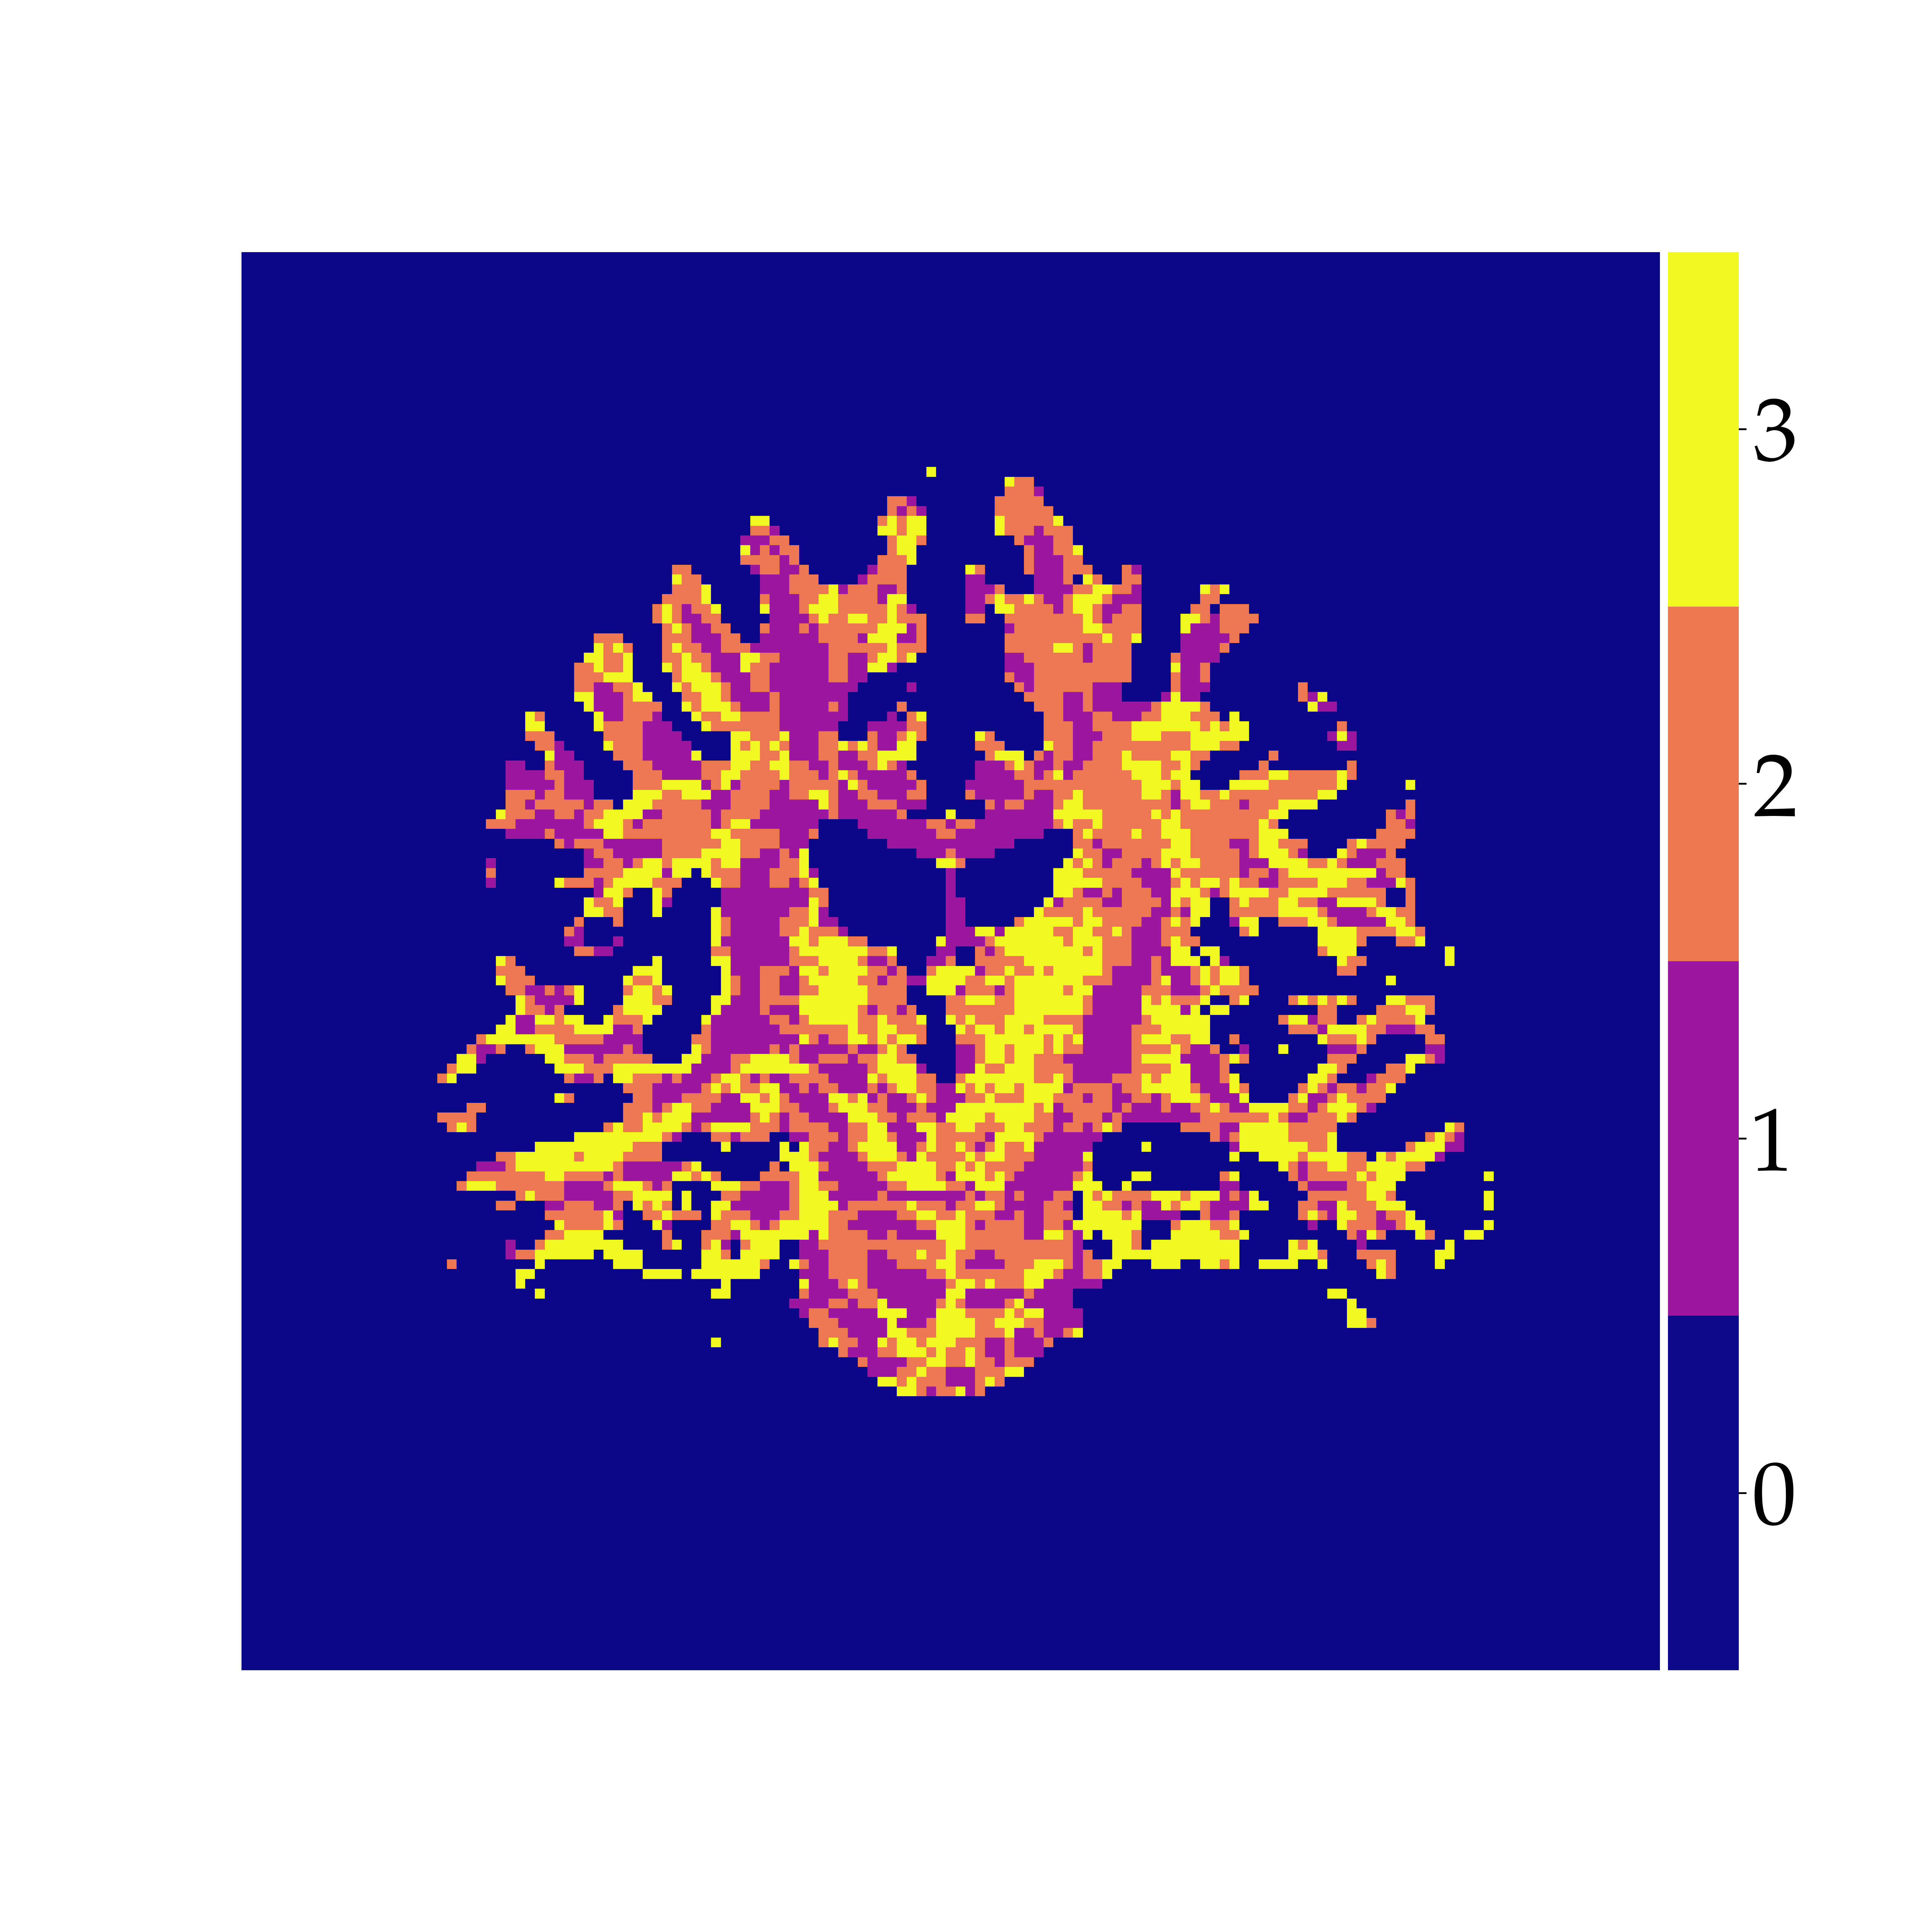
\includegraphics[width=\linewidth]{selected}
		\caption{The most likely number of fiber according to the
		selection model. {\color{white}asdfdsafdsfdsa}}
		\label{fig:selected-uncertainty:rank-original}
	\end{subfigure}
	\begin{subfigure}[b]{0.24\linewidth}
		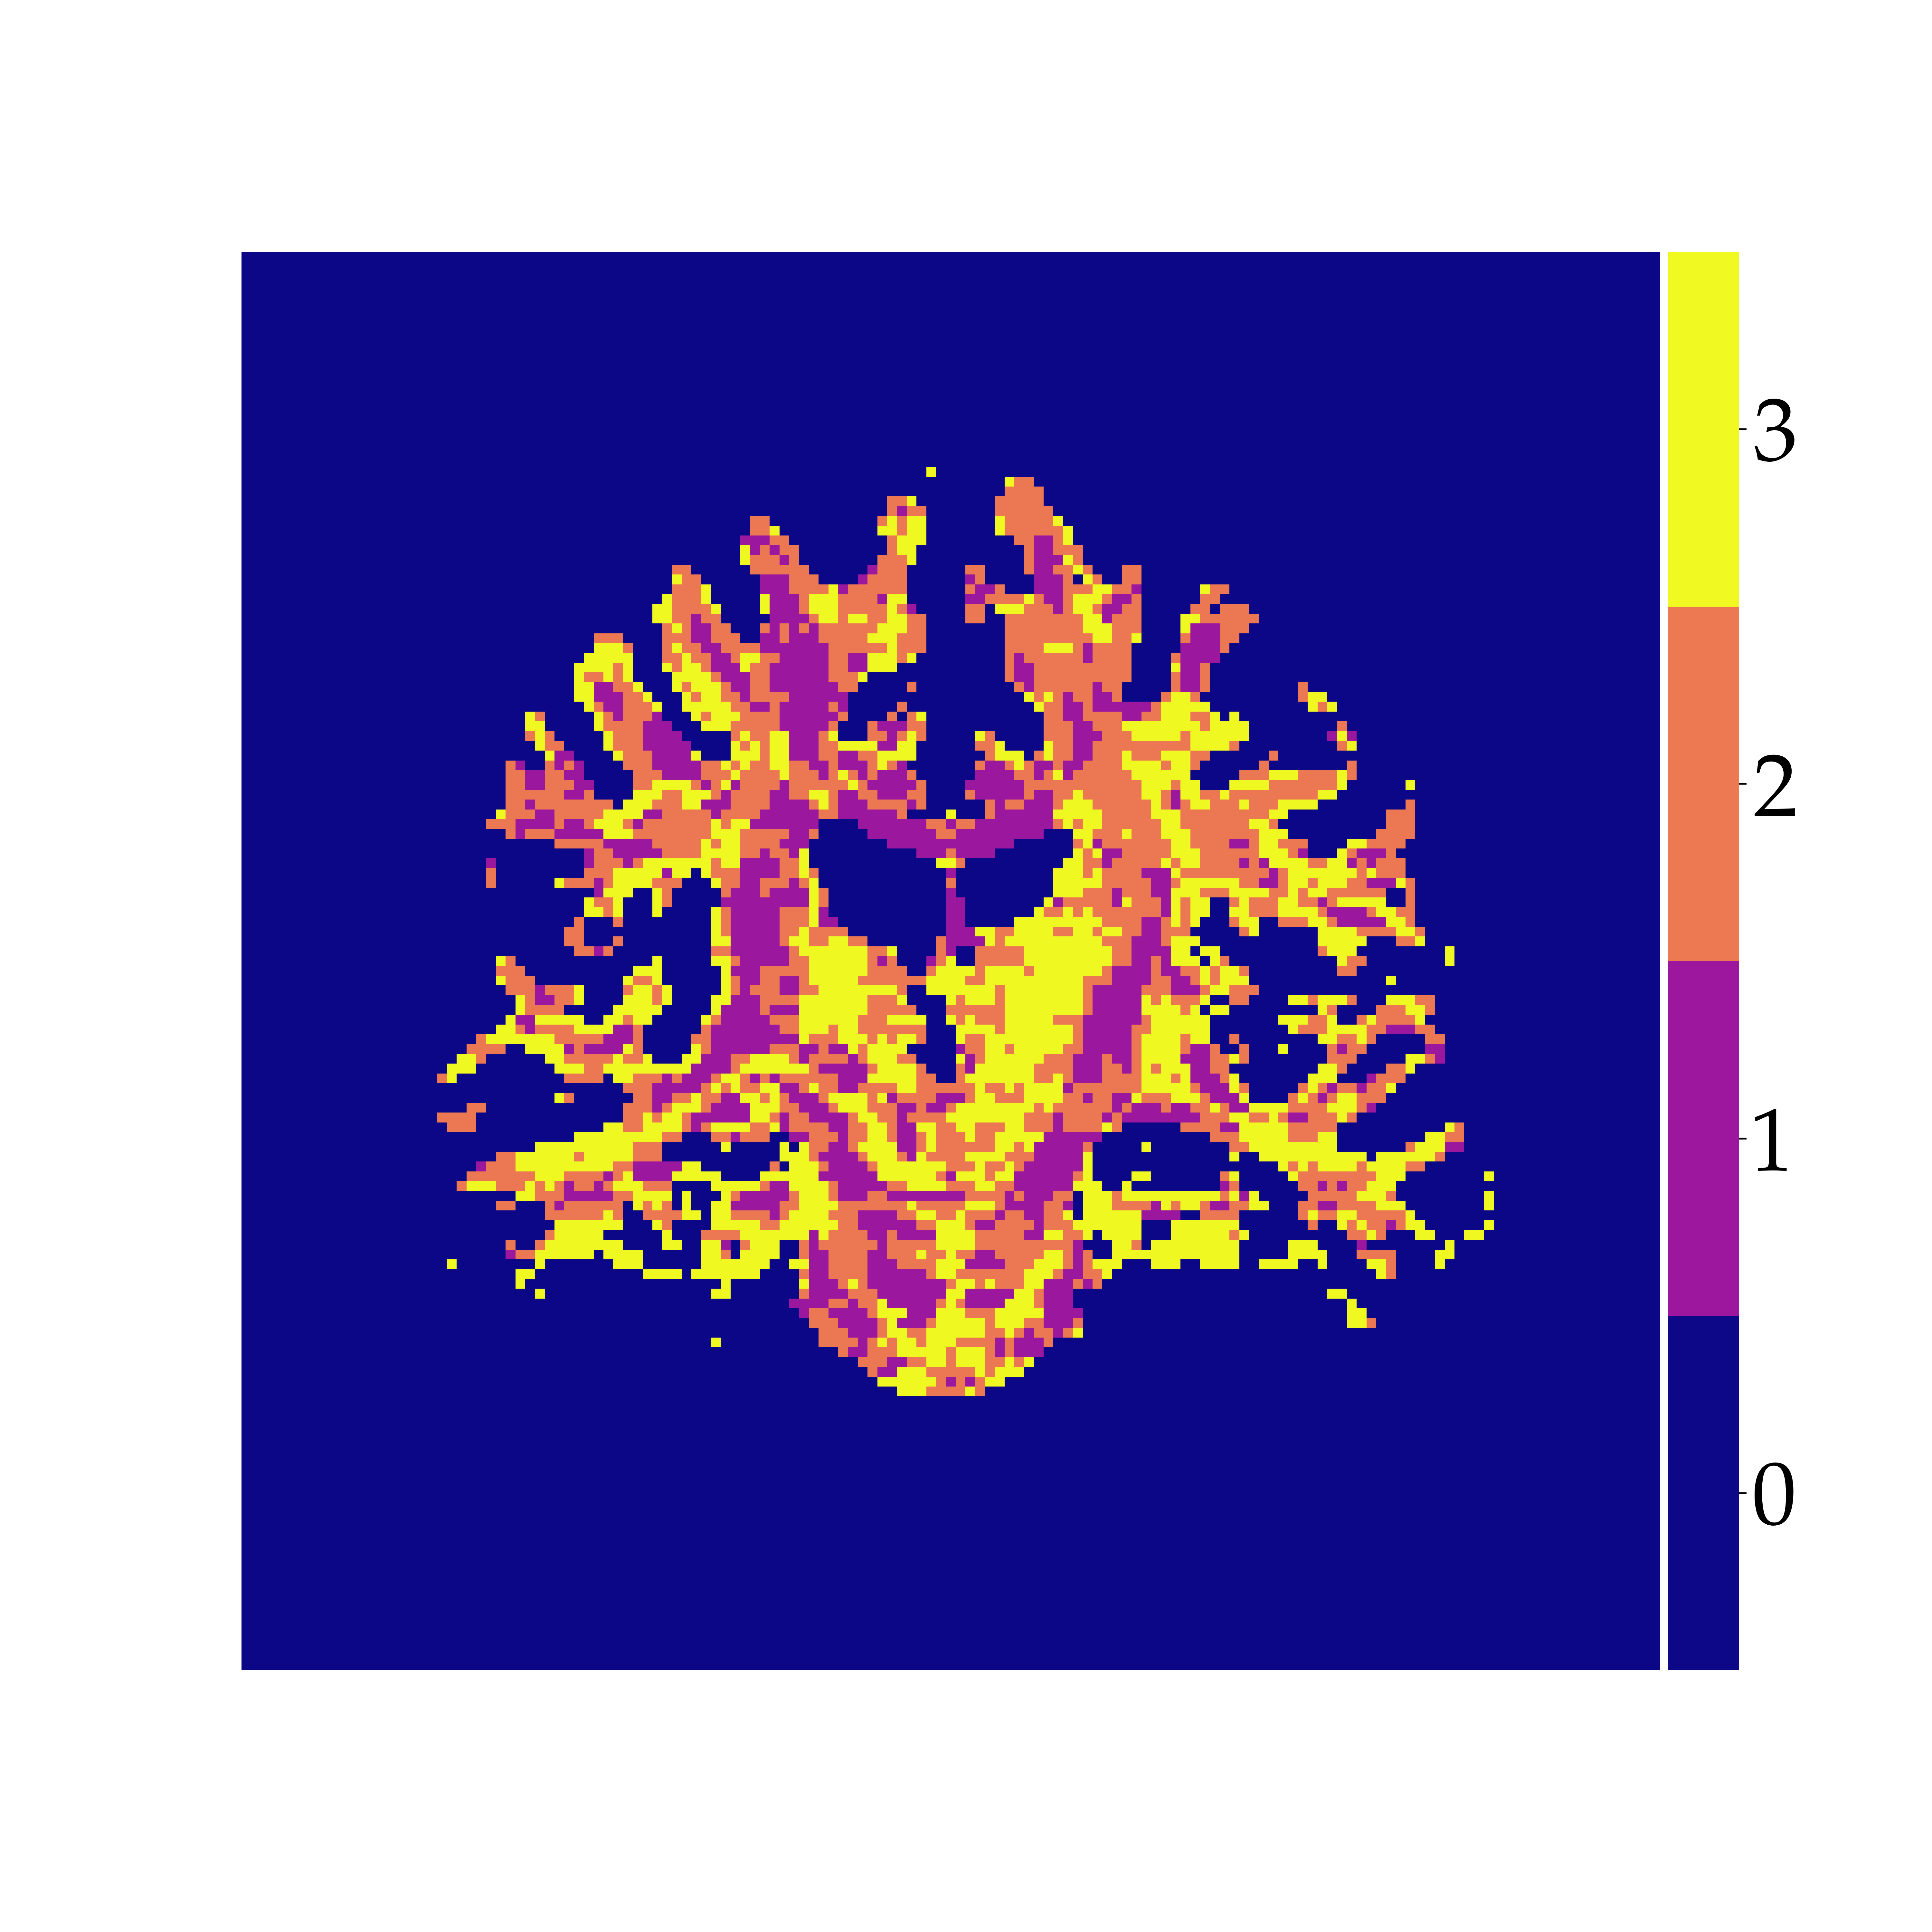
\includegraphics[width=\linewidth]{selected-bootstrap}
		\caption{The most like number of fibers over all
		bootstraps.{\color{white}iiiiiiiiiiii asdfdsafdsfdsa}}
		\label{fig:selected-uncertainty:rank}
\end{subfigure}  
	\begin{subfigure}[b]{0.24\linewidth}
		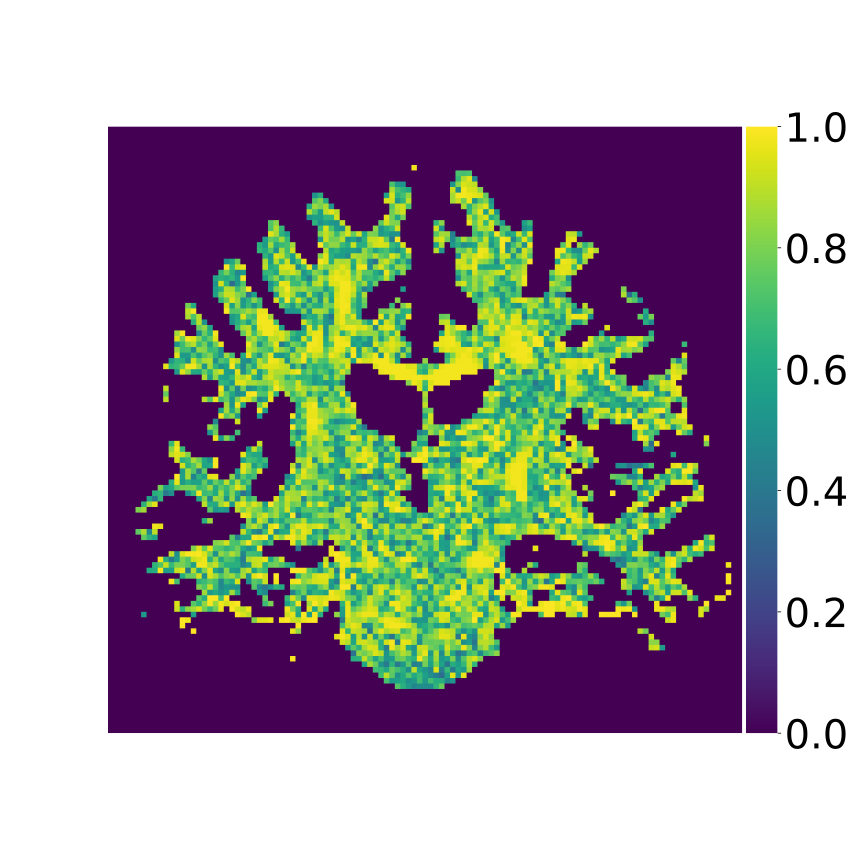
\includegraphics[width=\linewidth]{uncertainty}
		\caption{Certainty of the selected model.
		{\color{white}assdfsddfasd asdfdsafdsfdsa asdfsdafdfsfdfa}}
		
		\label{fig:selected-uncertainty:unc-original}
	\end{subfigure}
	\begin{subfigure}[b]{0.24\linewidth}
		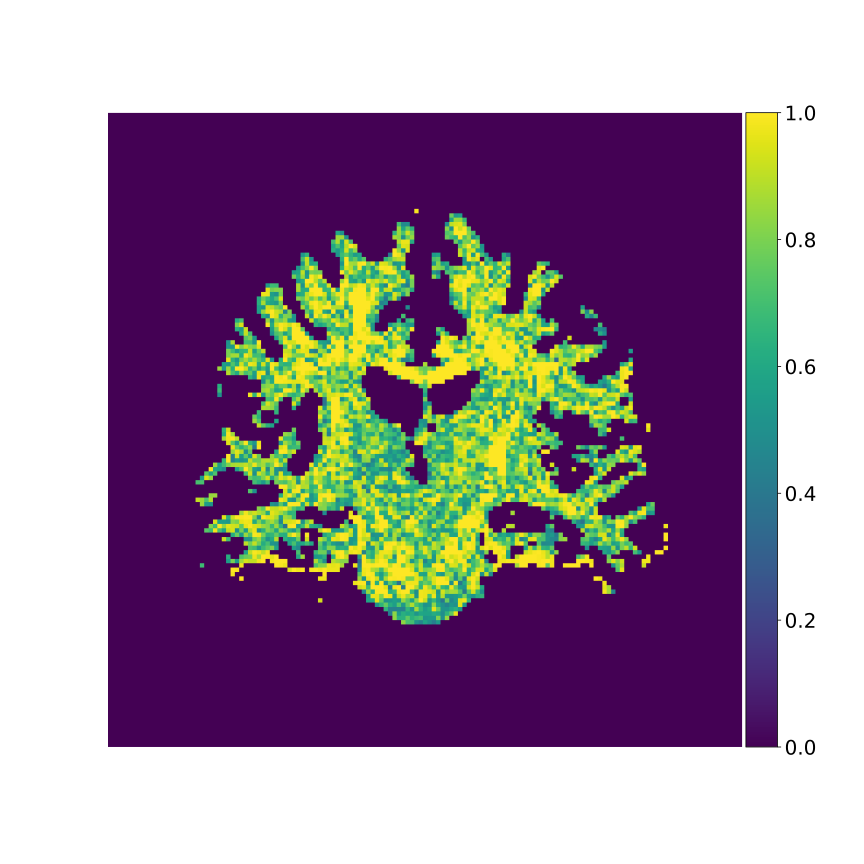
\includegraphics[width=\linewidth]{uncertainty-bootstrap}
		\caption{Number of bootstraps, which selected the most likely
		model over all bootstraps.}
		\label{fig:selected-uncertainty:unc}
	\end{subfigure}
	\caption{Comparison of model selection with and without bootstrapping.
	We denote that the Bayesian model is resistant against noise in the
sense that it selects in most cases the same model as the selection model
applied to the original data. However, it is also sensitive to noise, i.e. it
does not select always the same model.}
	\label{fig:selected-uncertainty}
\end{figure*}

Most bootstrap approaches in the context of dMRI are used  to generate
probabilistic tractographies out of deterministic tracking approaches. Such
approaches are reviewed in Section \ref{sec:related}. 

Our first novel contribution is to determine the uncertainty caused by
measurement errors to the proposed models in a systematical way. Therefore, wild bootstrapping is used to create
noisy resamples out of the measurements. The resampled data is then processed
and the parameters of a Watson distribution are evaluated to measure the
uncertainty which is propagated through the dMRI pipeline. 

As a second contribution we introduce a novel model, which reduces the measurement
uncertainty by incorporating all bootstraps into a new bootstrap consensus model.

\subsection{Wild Bootstrapping}
To evaluate the impact of measurement errors we use wild bootstrapping. It
has been shown in many cases that it is well suited within the context of dMRI and
is a straightforward way to
resample the original measurement without redoing the measurement process
\cite{Jones:2008}.

To create bootstrap samples the following process is applied. As a first step the model is fitted to the data. We obtain a fODF
$\hat{\mathcal{T}}$ and can calculate residual of Eq. (\ref{eq:sd-min}) 
\[ \hat{\varepsilon} = S - M\hat{\mathcal{T}} .\] 
A new bootstrap realization is calculated by 
\[ y^{*} = M\hat{\mathcal{T}}  + \hat{\varepsilon} v , \]
where $v$ denotes a random draw from the $n$ dimensional Rademacher distribution
\[ f \left( \mathbf{k} \right) \coloneqq  \begin{cases} \nicefrac{1}{2} \text{ if }
		\mathbf{k}_i=-1 \\
		\nicefrac{1}{2} \text{ if } \mathbf{k}_i=1 \\
		0 \text { otherwise } 
\end{cases} \text{ for } i \in \left\{ 1\dots n \right\} . \]
 Finally the model is fitted to the bootstrap realization. This process is repeated $m$
times to create a sample size of $m$ bootstraps.

For each sampled fODF we calculate the low-rank approximation of rank $3$
and with the obtained residuals also the selection and average model as it is
described in the previous section.

As a first contribution we investigate the distribution of the selected ranks
over all bootstrap. Therefore, we have simulated 100 bootstraps and applied the
selection model to all of them. The most
likely model in the original data is plotted in Fig.
\ref{fig:selected-uncertainty:rank-original} and the uncertainty of the selected model is
plotted in \ref{fig:selected-uncertainty:unc-original}. The generalization to the bootstrap model is
plotted right to the plots with the original data. Here the most likely number of fibers is
calculated by selecting the model, which occurs most in bootstraps. The count of
occurrences can be interpreted as uncertainty, e.g. if the selection model takes
always the same model not mattering the bootstrap errors, it is very certain
that this model fits the data well and vice versa.  
In most cases the selection model coincides with the most bootstraps. Only in
$14.1\%$ of the voxels withing the white matter area the selected rank differs
by $1$ and in $0.8\%$ the rank differs by $2$. Also regions which are quiet
certain are stay certain under bootstrapping. Therefore, we conclude that the
Bayesian posterior model is sensitive to noise and small changes in the data can
lead to different outcomes. 

\subsection{Bootstrap Consensus Model}
\begin{figure*}[t]
	\centering
	\begin{subfigure}[b]{0.33\linewidth}
		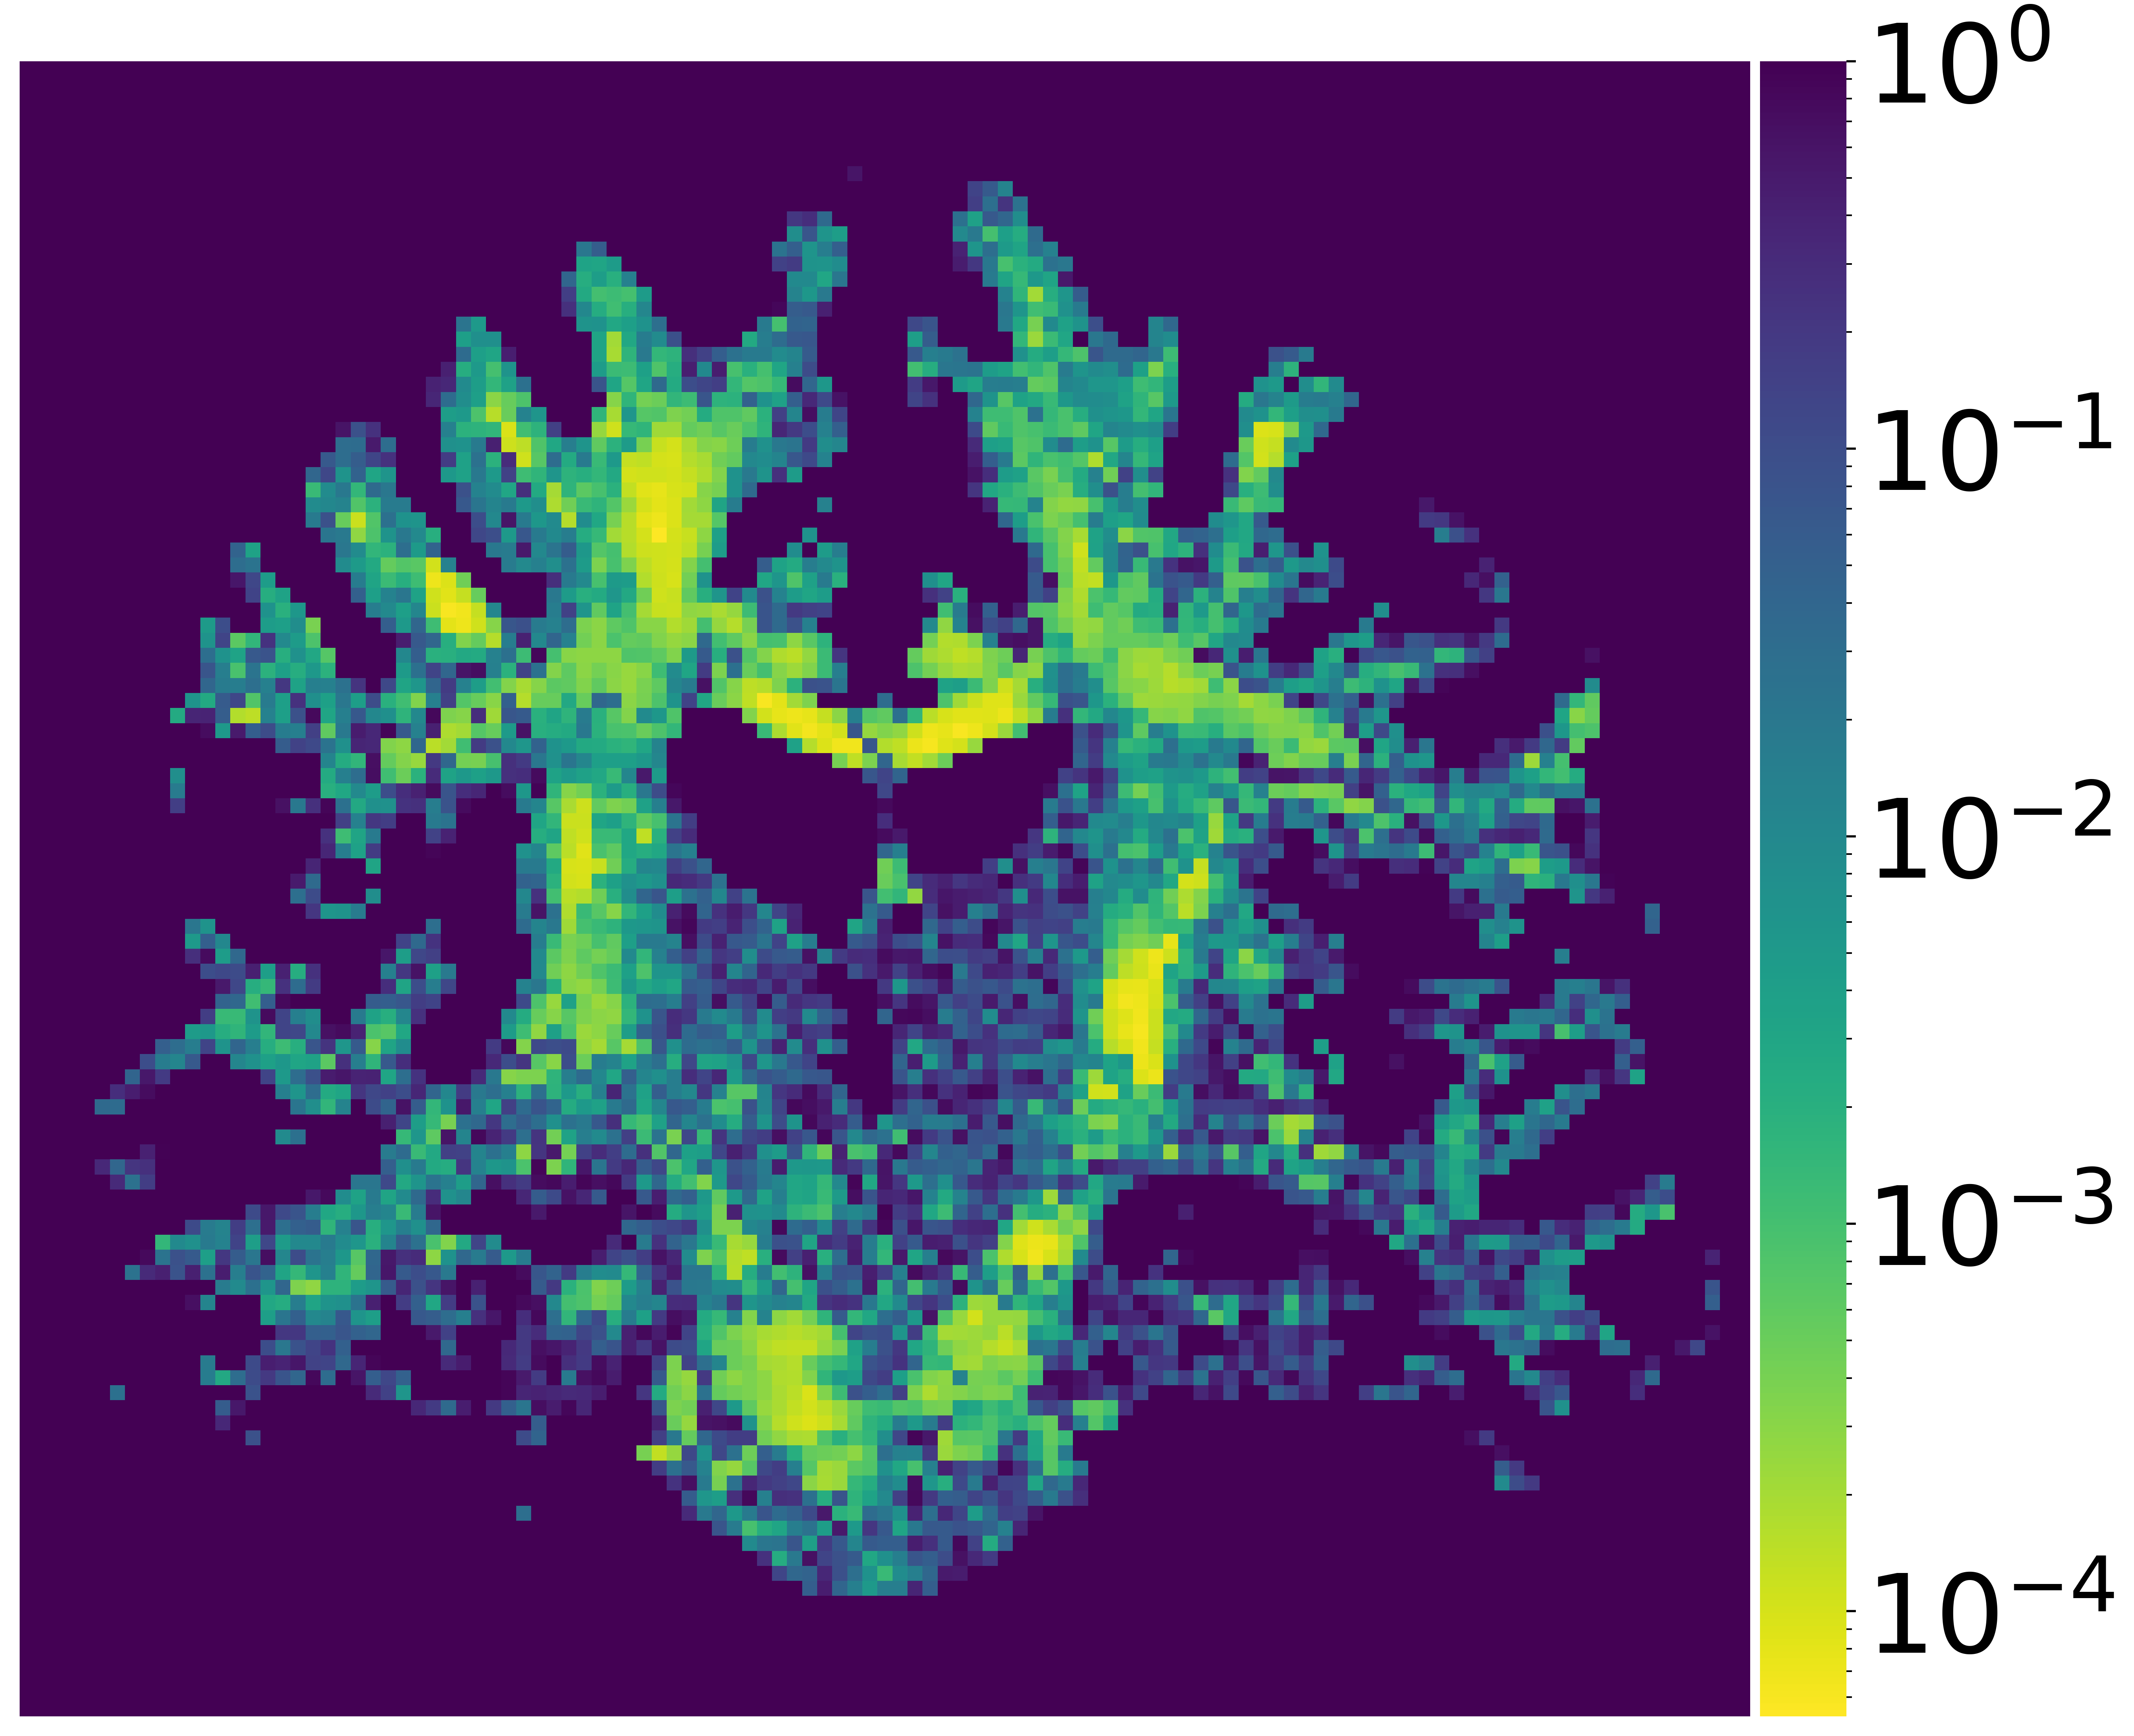
\includegraphics[width=\linewidth]{sel-bootstrap-maindir}
		\caption{Selection model}
		
	\end{subfigure}
	\begin{subfigure}[b]{0.33\linewidth}
		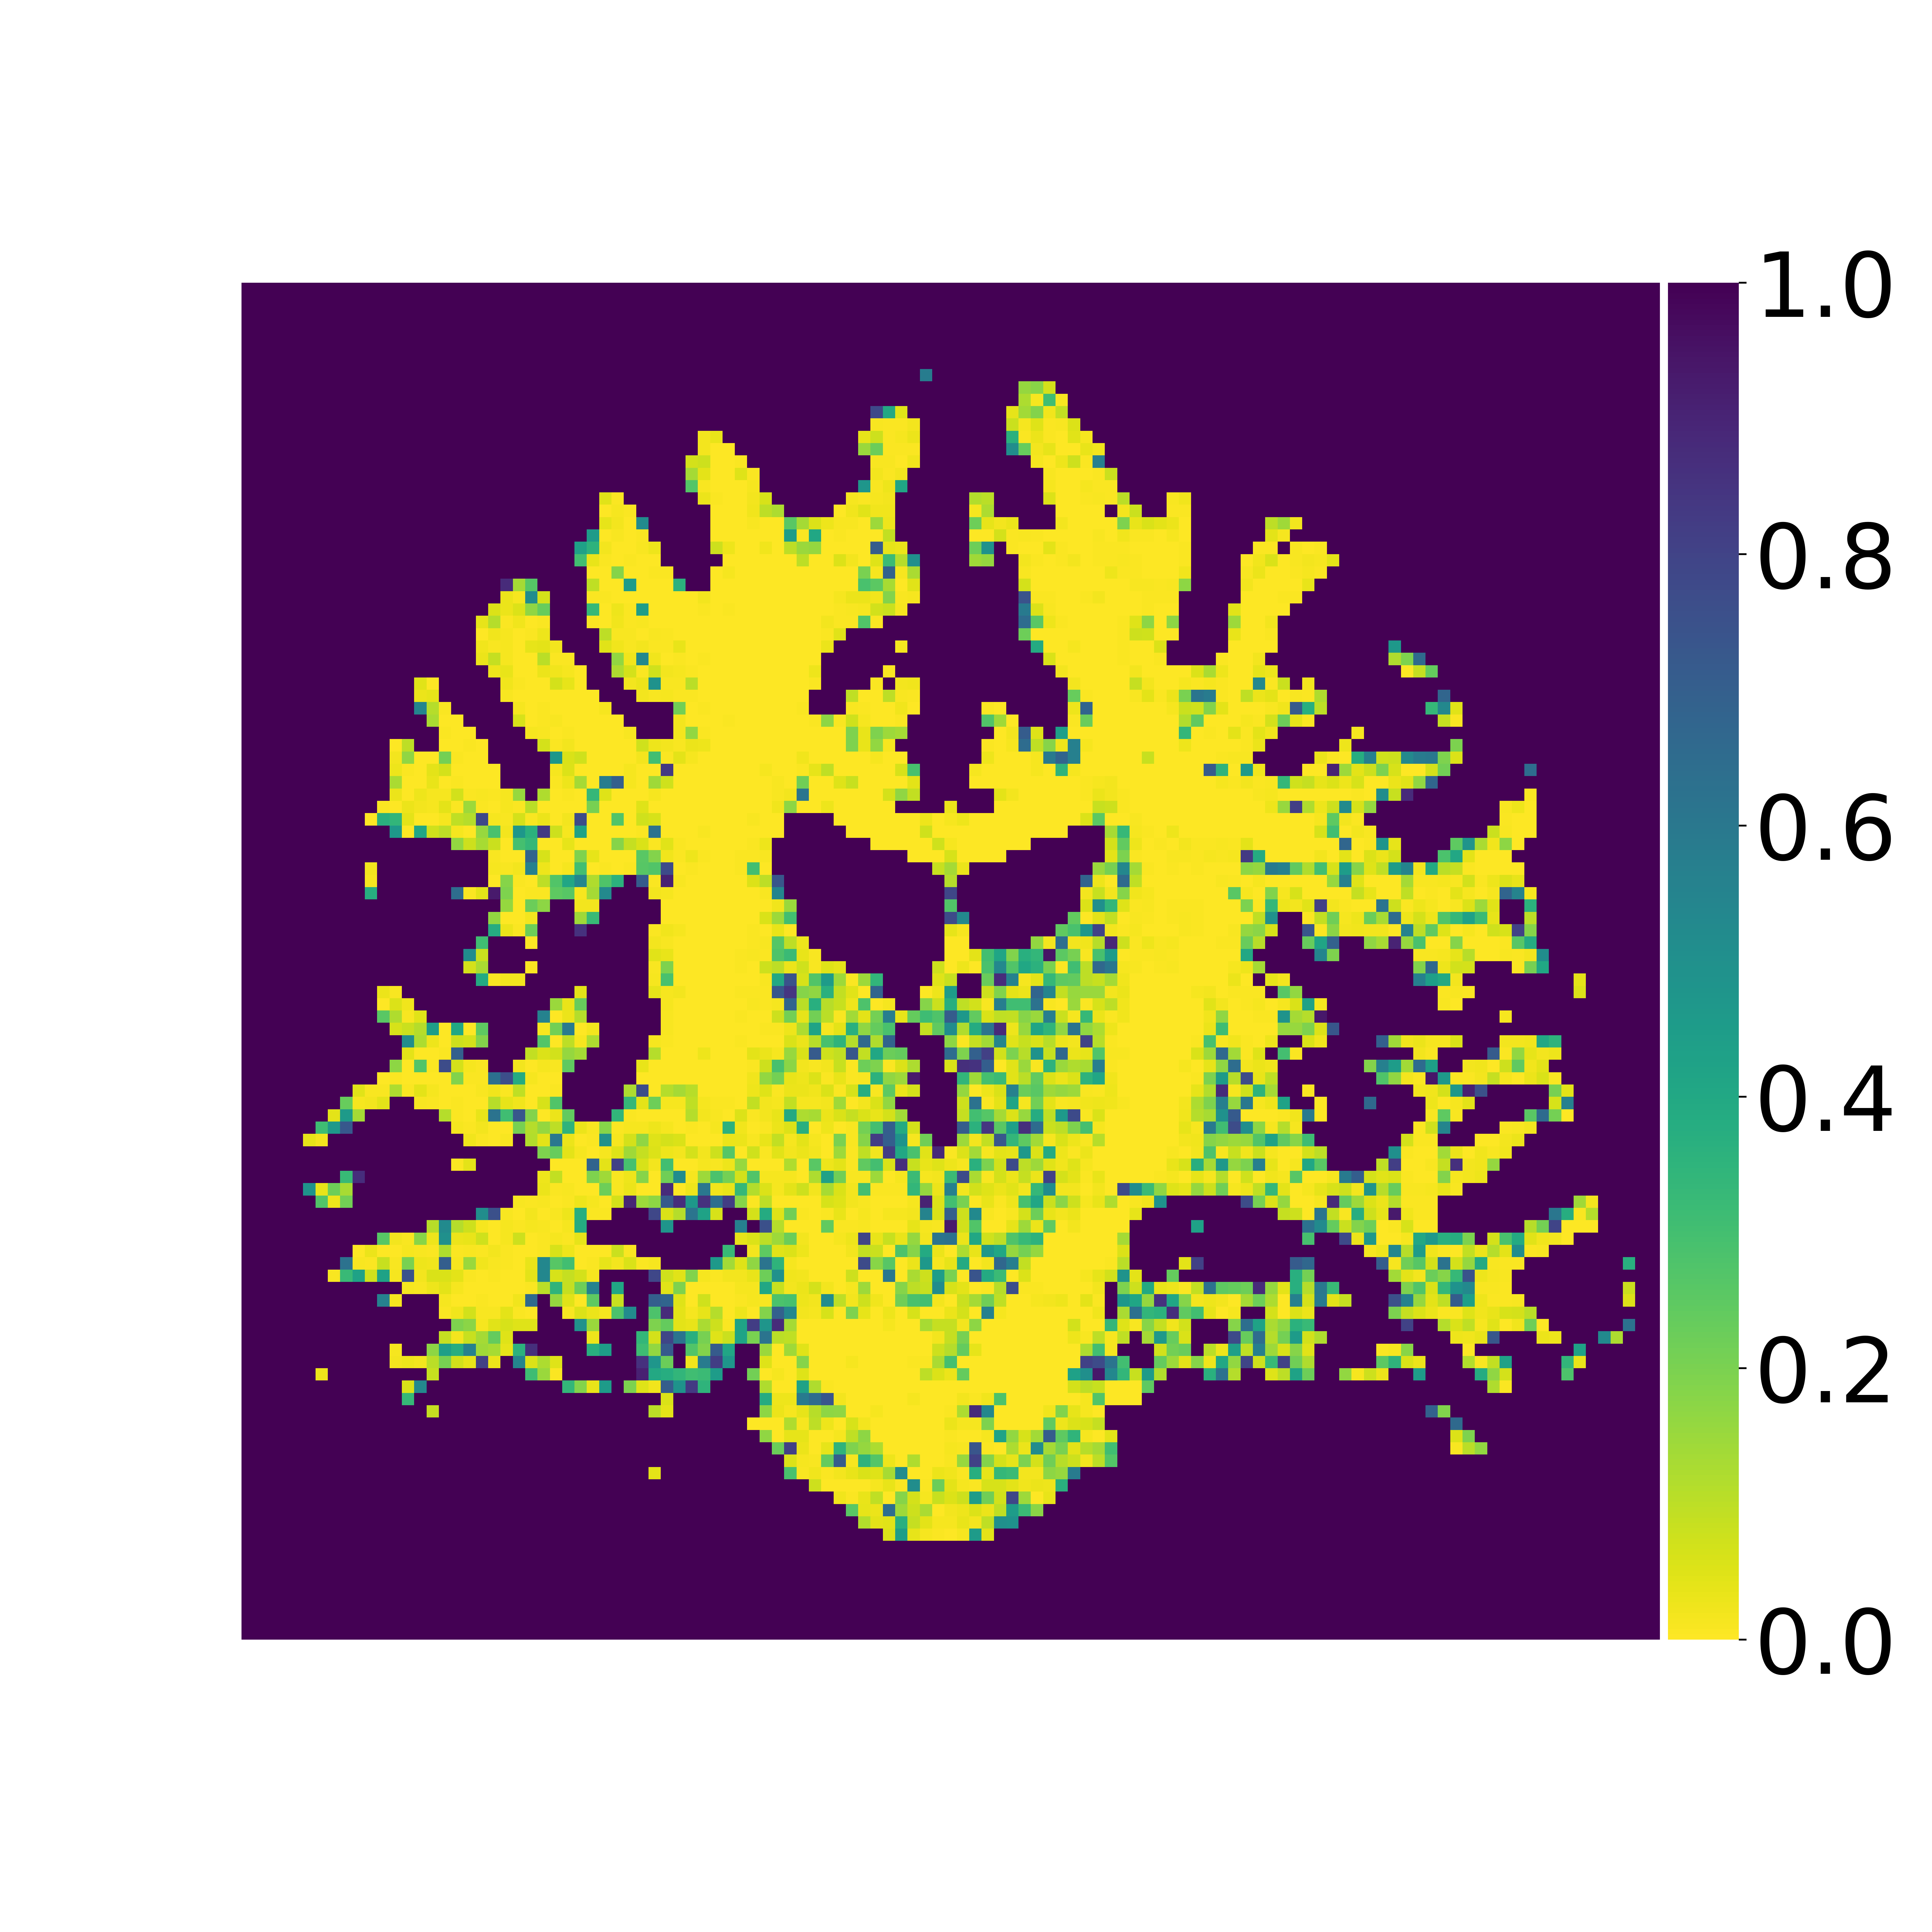
\includegraphics[width=\linewidth]{avg-bootstrap-maindir}
		\caption{Average model}
	\end{subfigure}
	\begin{subfigure}[b]{0.33\linewidth}
		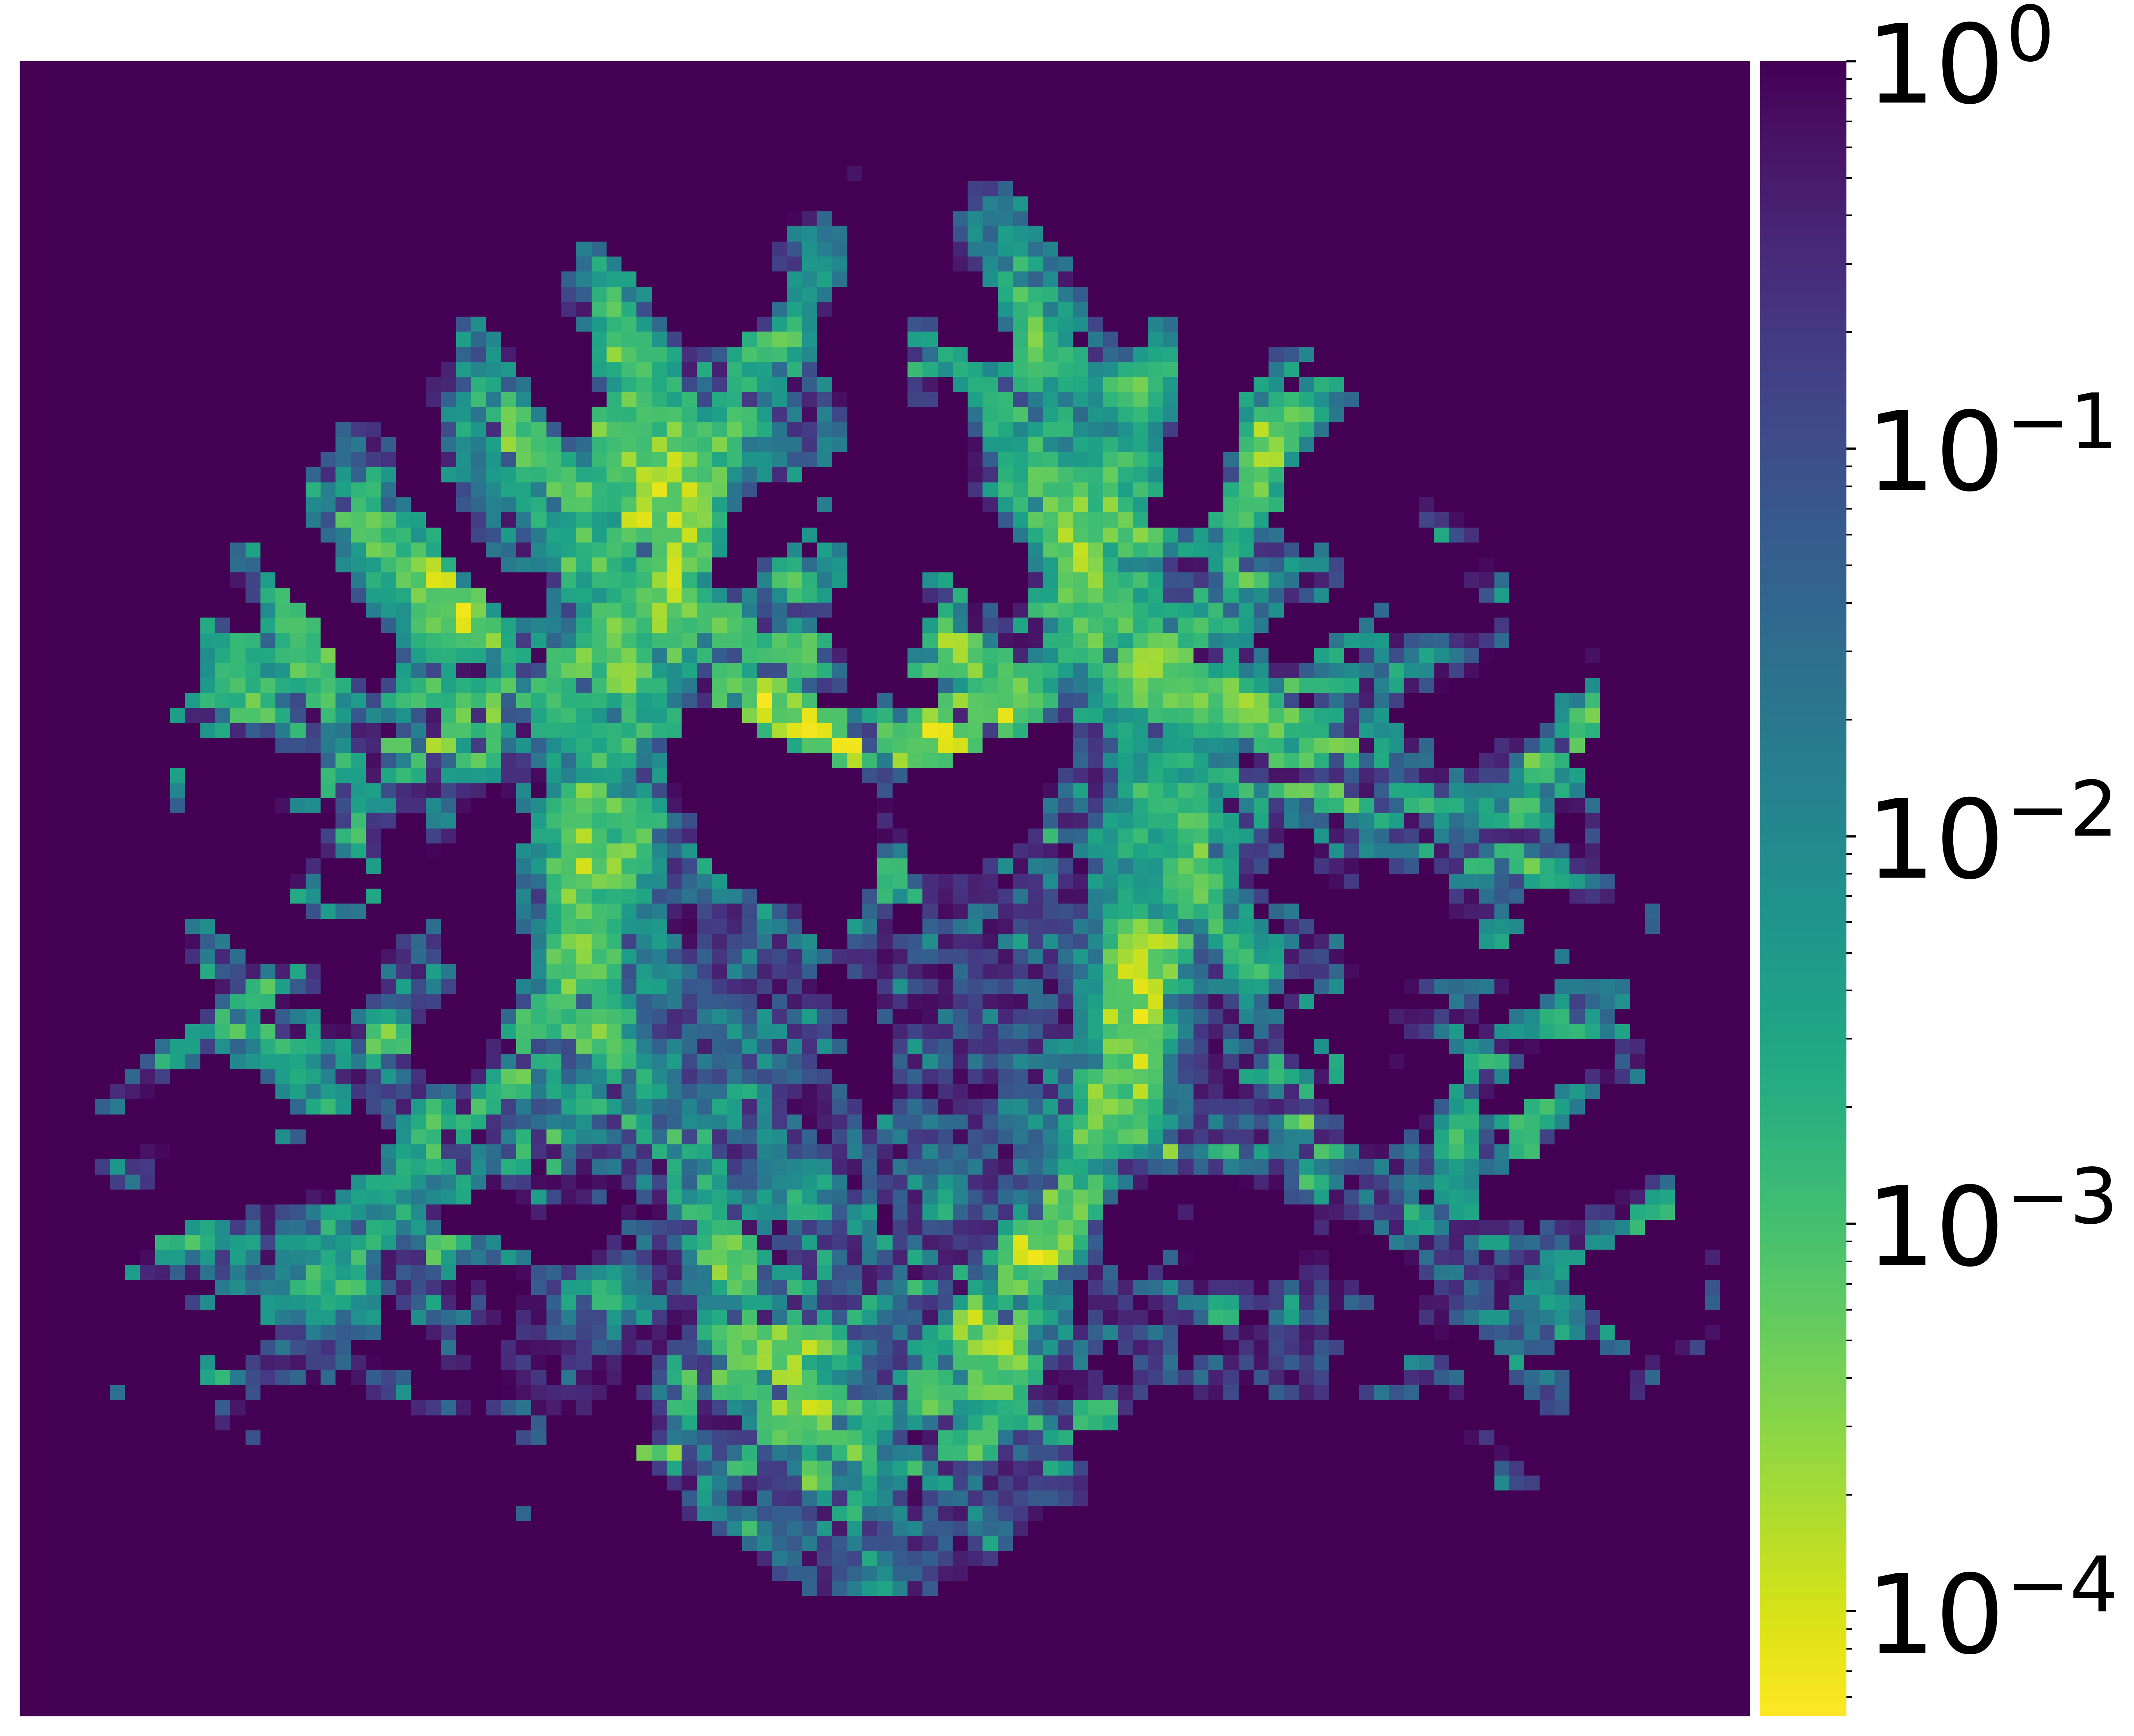
\includegraphics[width=\linewidth]{rank-bootstrap-maindir}
		\caption{Rank 3 model}
	\end{subfigure}

	\caption{Redefined orientation dispersion index calculated for the main
		direction (top row). The directions are ordered by volume fraction.
Within the main direction it is visible that the dispersion in the rank $3$
model is higher than in the both other models, which indicates a higher
susceptibility to noise. }
	\label{fig:dispersion}
\end{figure*}


Instead of using the bootstrap samples to produce a probability density map of
streamlines, we use it to reduce the measurement uncertainty by fusing the
information of all bootstraps into a new model. 
Therefore, the directions of all bootstraps get clustered to groups and the
group means are the new directions.

To build a consensus model we have to assign $n$ directions of $r$ bootstraps to $m$ groups on voxel
level where $m \geq n$. We initialize the process by setting the reference
direction for the $m$ groups as directions of
the low-rank $3$ model computed on the original data. Now each
direction of each bootstrap is assigned to a group such that the sum of
distances between group
reference and direction is minimized over all possible assignments to the
groups, i.e. we want to minimize the objective function 
\begin{align}
	T : \text{Sym} \left( n \right) & \mapsto \mathbb{R}_+ \nonumber \\
	Z & \rightarrow \sum \| \sgn \left( \langle \mathbf{v}_{Z\left( i
	\right)}, \bar{\mathbf{v}}_i \rangle \right) \mathbf{v}_{Z\left( i
	\right)} - \bar{\mathbf{v}}_i\| ,  
\end{align} 
where $\text{Sym}\left( n \right)$ denotes the symmetric group, 
$\bar{\mathbf{v}}_i$ denotes
the reference direction and $\mathbf{v}_i$ denotes the direction from the
bootstrap. To prevent wrong assignments if only one reference
direction is initialized we first assign the direction from the bootstrap with
the  highest fiber count to the
groups and update the uninitialized reference directions with the assignments.
Note that this does not necessary lead to a global optimum, but is in most cases
close to the optimum. 

To get deeper insights into the impact of the bootstrapping we fit a Watson
distribution to the grouped directions \cite{jupp_mardia_1999}. The Watson distribution is defined as  
\begin{align*}
	f : \mathbb{S}^2 & \longrightarrow  \mathbb{R}_+ \\
	\mathbf{x} & \longmapsto  M \left( \frac{1}{2}, \frac{3}{2} , \kappa
	\right)^{-1} \exp \left(  \kappa
	\left( \mathbf{\mu}^T \mathbf{x} \right)^2 
	\right) 	,  
\end{align*}
where $\kappa$ is the dispersion parameter, $\| \mathbf{\mu} \| = 1$ the
mean direction and $M$ be the confluent hypergeometric function. 

We use the Watson distribution because it has two main advantages. First of all, it is antipodal symmetric,
which fits our model assumption of indistinguishable $\pm \mathbf{v}$
directions. Secondly, it is one of the easiest models for axial data and
introduces the dispersion parameter, which gives  us deeper insights into the
uncertainty within the groups. 

In Fig. \ref{fig:dispersion} we have visualized the redefined orientation dispersion index
\cite{dispersionParameter}  
\[ OD = \frac{2}{\pi} \arctan \left( \frac{1}{\kappa} \right) \] 
for the selection, average and rank 3 model. This score is more intuitive since
it maps the low dispersion to low values and vice versa. 

It is visible that the
selection model and average model shows lower dispersion in large parts of the CC and CST tracts
compared to the rank $3$ model. This is caused by the
ability of the selection model to select the rank $1$ model in this areas, which
is not as susceptible to noise as higher rank models. I.e. the selection model
reduces the impact of measurement noise without explicitly being build for
this. The average model also benefits from the noise reduction, since the impact
of the lower rank models is high in these regions.
On the other hand the average model still contains more fiber directions, which
makes it more flexible compared to the selection model, which contains in many
voxels just a single fiber direction.
We conclude that average model fuses the stability from the selection model in
the mean direction and also the flexibility of the rank $3$ model, which can be
important in crossing regions.
Therefore, we assume that the impact to the average and rank $3$ model is lower
than to the selection model since we increase the flexibility by introducing
more directions into the consensus selection model. 



%%% Local Variables:
%%% mode: latex
%%% TeX-master: "../main"
%%% End:

\section{Crossing Fiber Tractography with Reduced Measurement Uncertainty}

\subsection{Probabilistic Streamline-Based Tractography}

Within this work a probabilistic streamline-based approach is used. For a given
seed point, the streamline grows iteratively in both directions using Euler
integration. Since neither the seed point nor any other point of the streamline
lies on a grid point, we interpolate the current position trilinearly. Therefore,
we have to solve a matching problem first, since we have to decide which
directions belong together to apply the trilinear interpolation. Since we assume
smoothness between the voxels we use the three directions, from the last
interpolation step as group means $\bar{\mathbf{v}}_i$, $i \in \left\{ 1\dots 3 
\right\}$. Now we fit each vertex to the group means such
that 
\begin{align}
	\text{Sym} \left( r  \right) & \rightarrow \mathbb{R}_+ \\ 
	Z & \mapsto \sum \| \sgn \left( \langle \mathbf{v}_{Z \left( i \right)}
	, \bar{\mathbf{v}}_i \rangle  \right) \mathbf{v}_{Z \left( i \right)} -
\bar{\mathbf{v}}_i
	\|
\end{align}
is minimized. We only update the group means if a group mean is not defined.
Then we solve the above minimization problem and assign the direction as new
group mean. Afterwards, we rerun the minimization for all vertices. This is done,
to reduce the time consumption drastically. Further, the local optimal
configuration is cached. Using this, we only have to calculate the assignments
once for each voxel which we are tracking through. 
To initialize the trilinear interpolation, we take the directions of the nearest voxel as group means.
Given the interpolated directions $\mathbf{v}_i$ at the current point, we
reorient them to have a non-negative inner product with the current tracking
direction $\mathbf{w}$. We select one of the $r$ possible directions by the
following probabilistic model.

We assign each unit direction $\mathbf{v}_i$ with the volume fraction
$\lambda_i$ for $i \in \left\{ 1\dots r \right\}$ following the probability
scheme 
\[
	p \left( \mathbf{v}_i \right) \coloneqq \frac{ \mathbb{1}_{\lbrace\theta_i <
		\frac{1}{3} \pi \rbrace} \lambda_i \cos \left( \left( \frac{3}{\sqrt{2
\pi}} \theta_i \right)^2 \right)}{\sum_j \mathbb{1}_{\lbrace\theta_j <
		\frac{1}{3} \pi \rbrace} \lambda_j \cos \left( \left( \frac{3}{\sqrt{2
\pi}} \theta_j \right)^2 \right) }, 
\]
where $\theta_i$ denotes the angle between the possible direction $\mathbf{v}_i$
and the current direction $\mathbf{w}$. 

The proposed probability function assigns angles below 30 degrees almost the
same probability, which coincides with the limited angular resolution of
spherical deconvolution \cite{TOURNIER20071459}. Further, the maximum angle is
restricted to 60 degrees, which coincides with our anatomical knowledge.

This iterative algorithm proceeds until we either reach a region with fractional
anisotropy below $0.3$ or the summed angle over the last $30$ mm is greater than
$130$ degrees. This prevents streamlines to go back and forth. 

\subsection{Postprocessing}
While diffusion MRI is in general able to reconstruct large parts of the white
matter tracts, it is also well known that it is suspiscious to reconstruct false
positives, which have to be removed according to anatomic knowledge
\cite{Wakana:2007, MaierHein:2017}. Further, the probabilistic tracking approach
generates outliers with low density, which have to be removed to have a proper
output. 

To avoid false positives, we use inclusion and exclusion regions. All regions
are set carefully for a reference patient according to [hier die quelle].
The remaining patients are linearly registered to the reference patient and the
linear transformation is used to map the regions to the other patients. 
If a streamline intersects with an exclusion region, the whole streamline is
discarded and if a streamline does not intersect with all inclusion regions, it
is discarded as well. 

Further, we create a density map for each streamline
bundle. Therefore, we count the number of streamlines intersecting each voxel.
All streamlines are cut off at the first intersection with a low density
area starting from the seed. The low density threshold is also defined for the
reference patient and then mapped to all other patients according to the seed
ratio.

\section{Results}
\subsection{Data}
The proposed novel consensus model is applied to the selection,
average and rank $3$ model. The CSD model got replaced by the rank $3$ model
because it was knocked off compared to the other models by Dice score. Further,
the CSD used in the model is computational heavy, i.e. computation takes 4 times as long
as the $4$th order CSD which is used within this paper. This especially matters
because of the time intense bootstrap creation. 

To evaluate the proposed models, data from the Human
Connectome Project (HCP) is used \cite{HCP}. The diffusion MR images have a resolution of $1.25$ mm
isotropic with $145 \times 174 \times 145$ voxels. 

As reference data we use the high quality data, which was published within the
scope of the Tractseg paper \cite{WASSERTHAL2018239}. This reference data has been
created by manually refining the segmented full brain fiber tractography. For
more details we refer to the original literature.

All tests were performed on 12 randomly chosen subjects for which such reference tractographies
exist. For each tract we created seed points by intersecting the reference
fiber bundle with a plane and initialize the tracking process with the direction
of the fiber bundle at the seed point. This should mimic a directional region of
interest as it might be defined by an expert on brain anatomy
\cite{Graumann2016}. We then apply the tracking process until we have as many
streamlines as the reference tractography. This should guaranty that the
comparison between the different models is fair.

\subsection{Qualitative Comparison}
\begin{figure}[t]
	\centering
	\begin{subfigure}[b]{0.45\linewidth}
		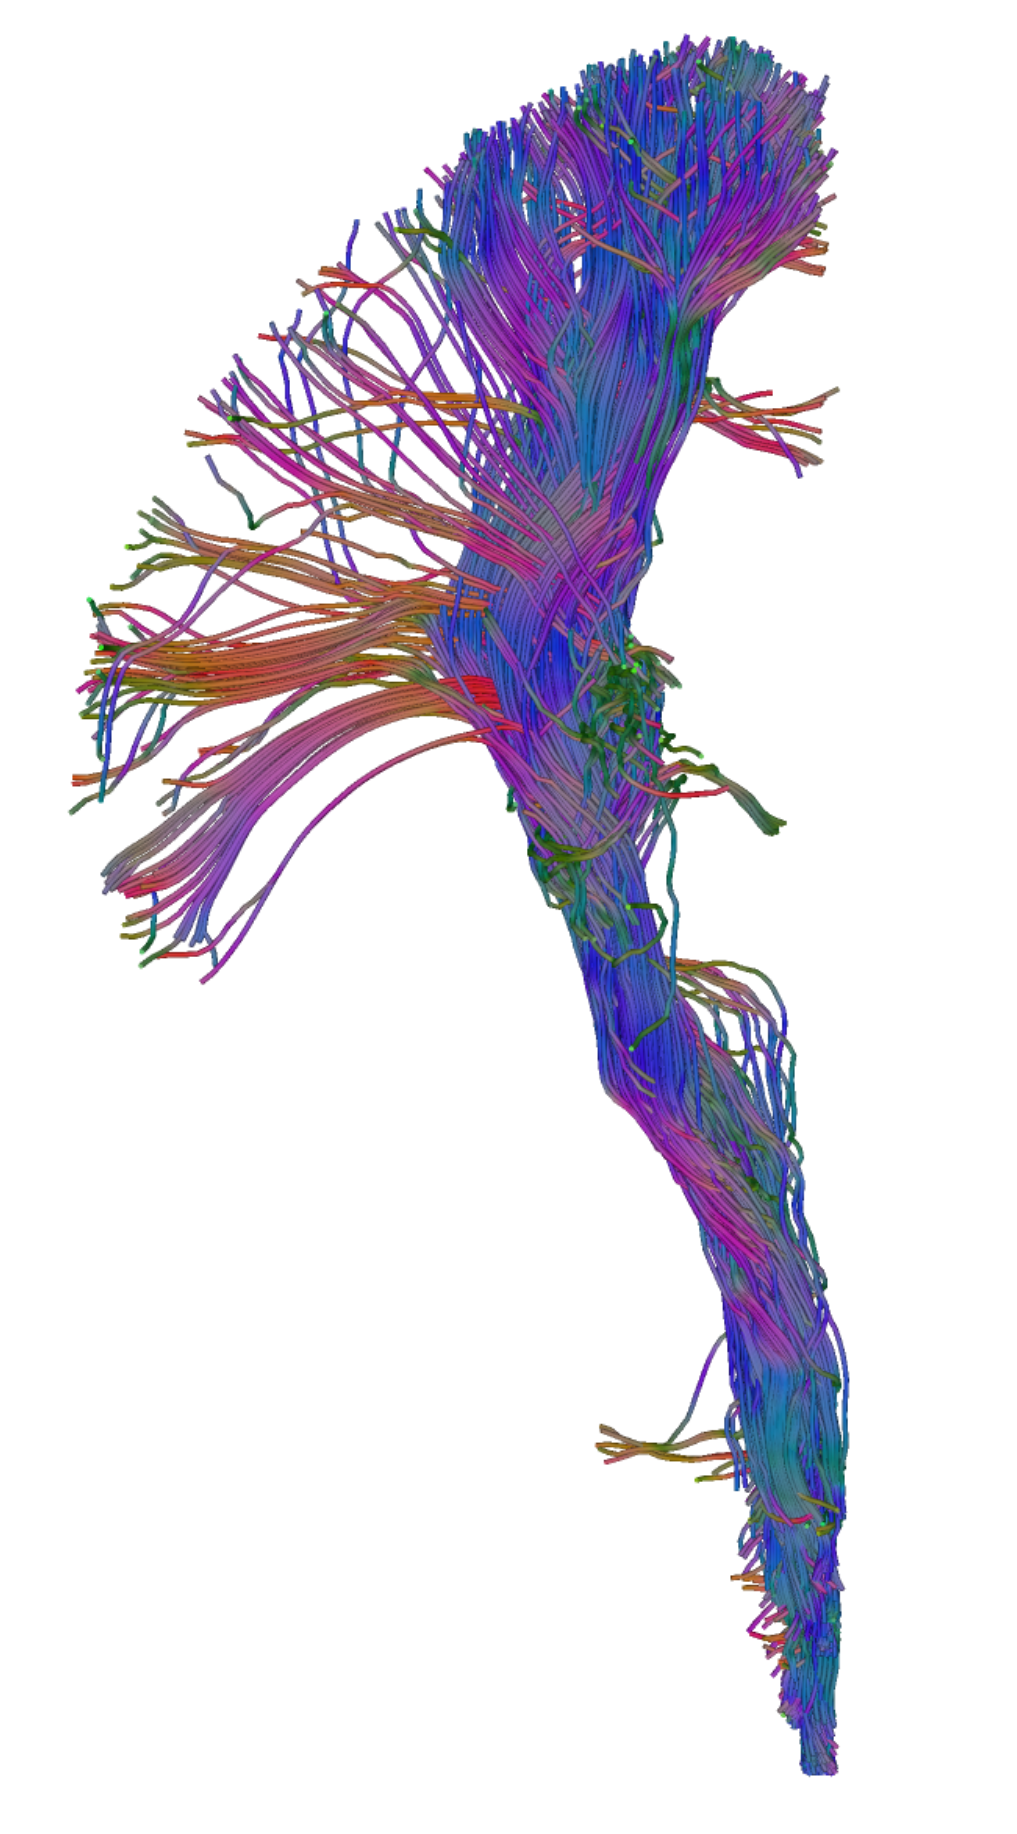
\includegraphics[width=\linewidth]{cst-rank-c}
		\caption{Low rank 3 model}
	\end{subfigure}
	\begin{subfigure}[b]{0.45\linewidth}
		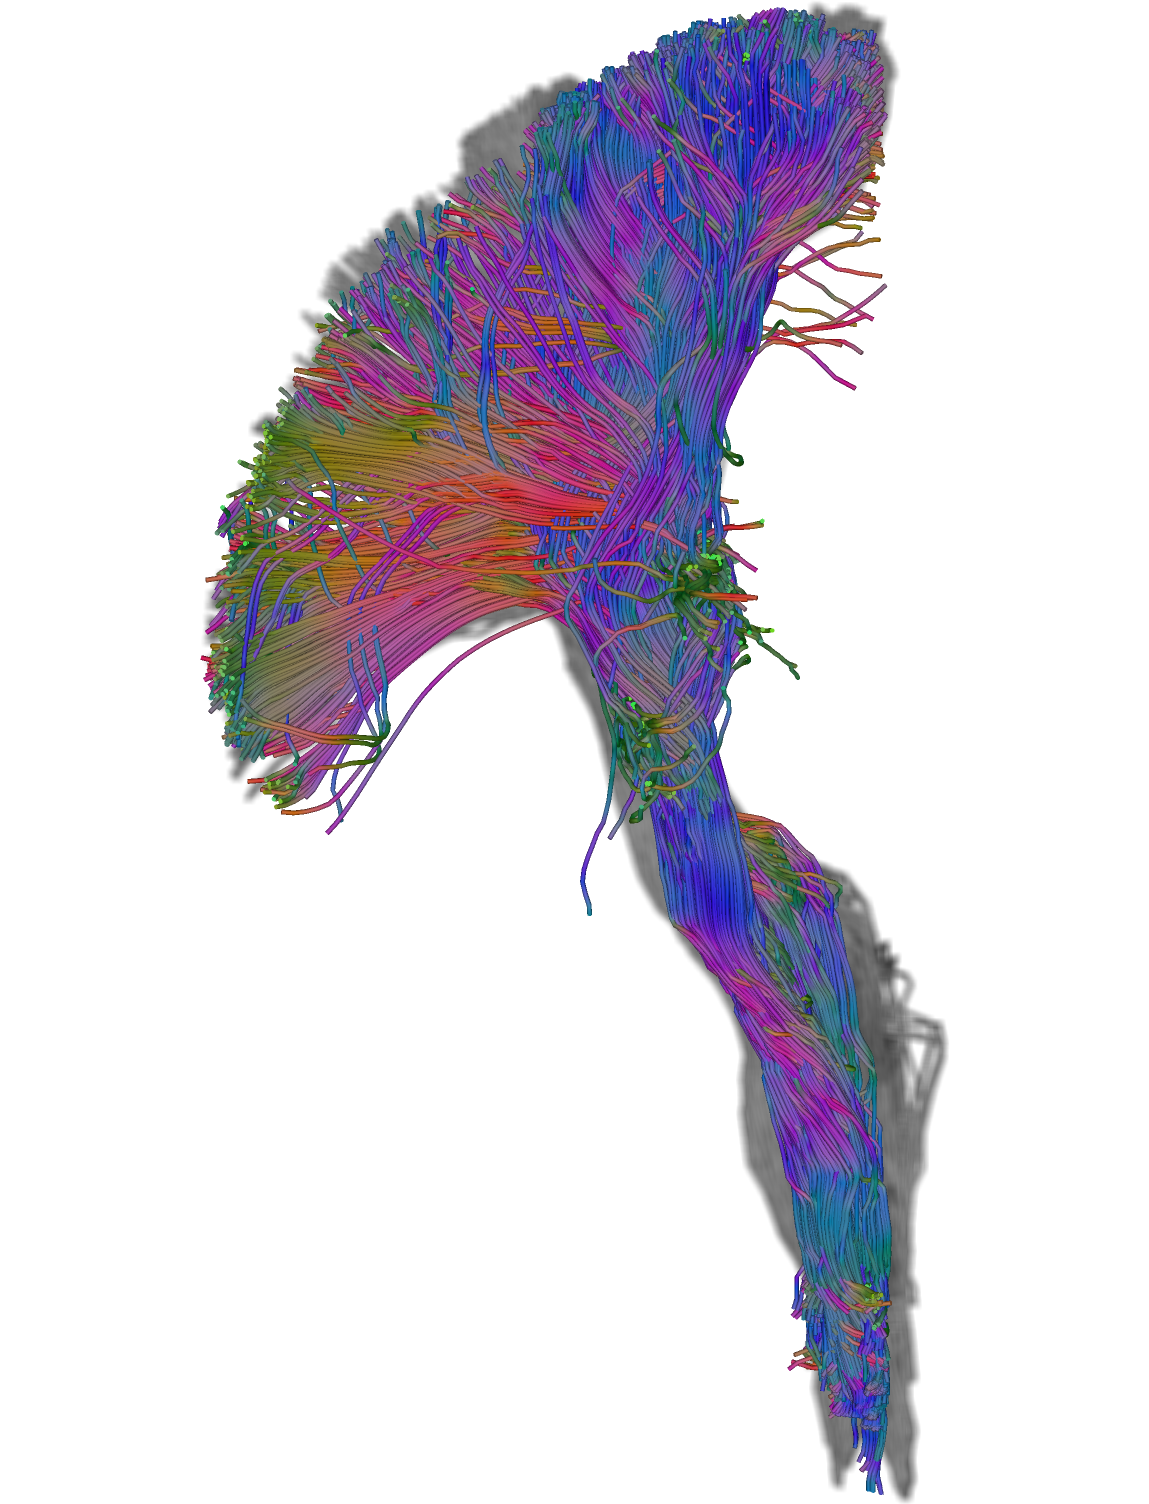
\includegraphics[width=\linewidth]{cst-rank-bootstrap-c}
		\caption{Consensus low rank 3 model}
\end{subfigure} \\
	\begin{subfigure}[b]{0.45\linewidth}
		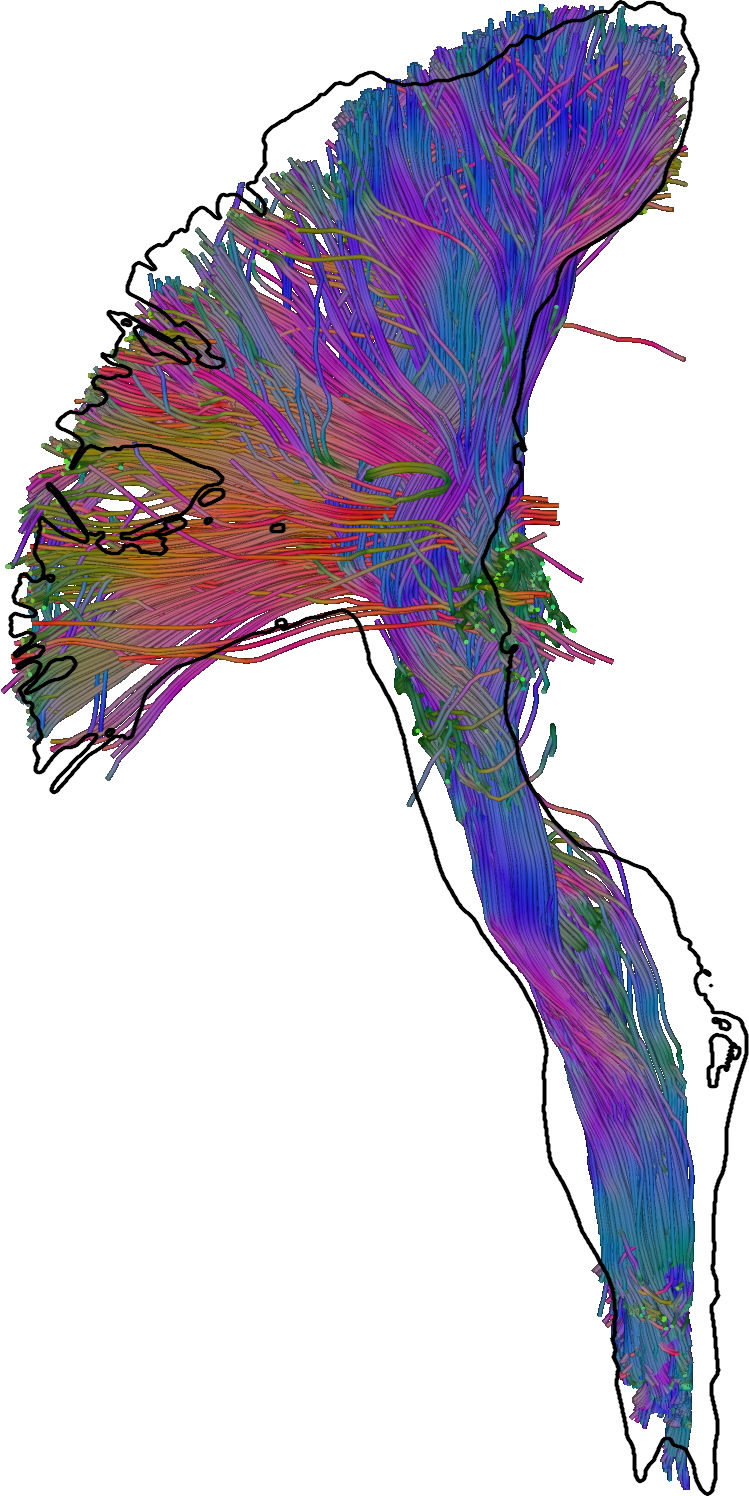
\includegraphics[width=\linewidth]{cst-avg-c}
		\caption{Average model}
	\end{subfigure}
	\begin{subfigure}[b]{0.45\linewidth}
		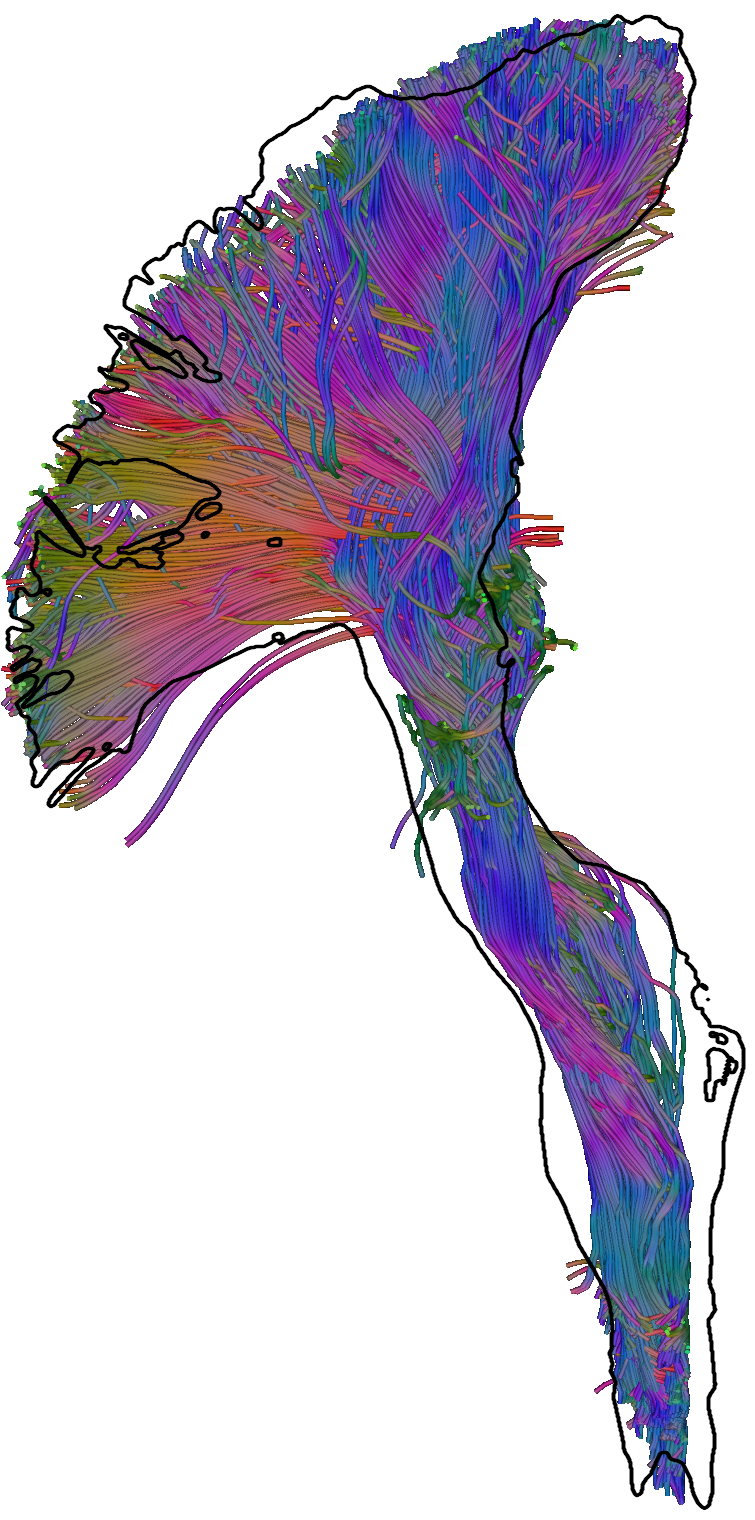
\includegraphics[width=\linewidth]{cst-avg-bootstrap-c}
		\caption{Consensus Average model}
\end{subfigure} \\
\begin{subfigure}[b]{0.45\linewidth}
		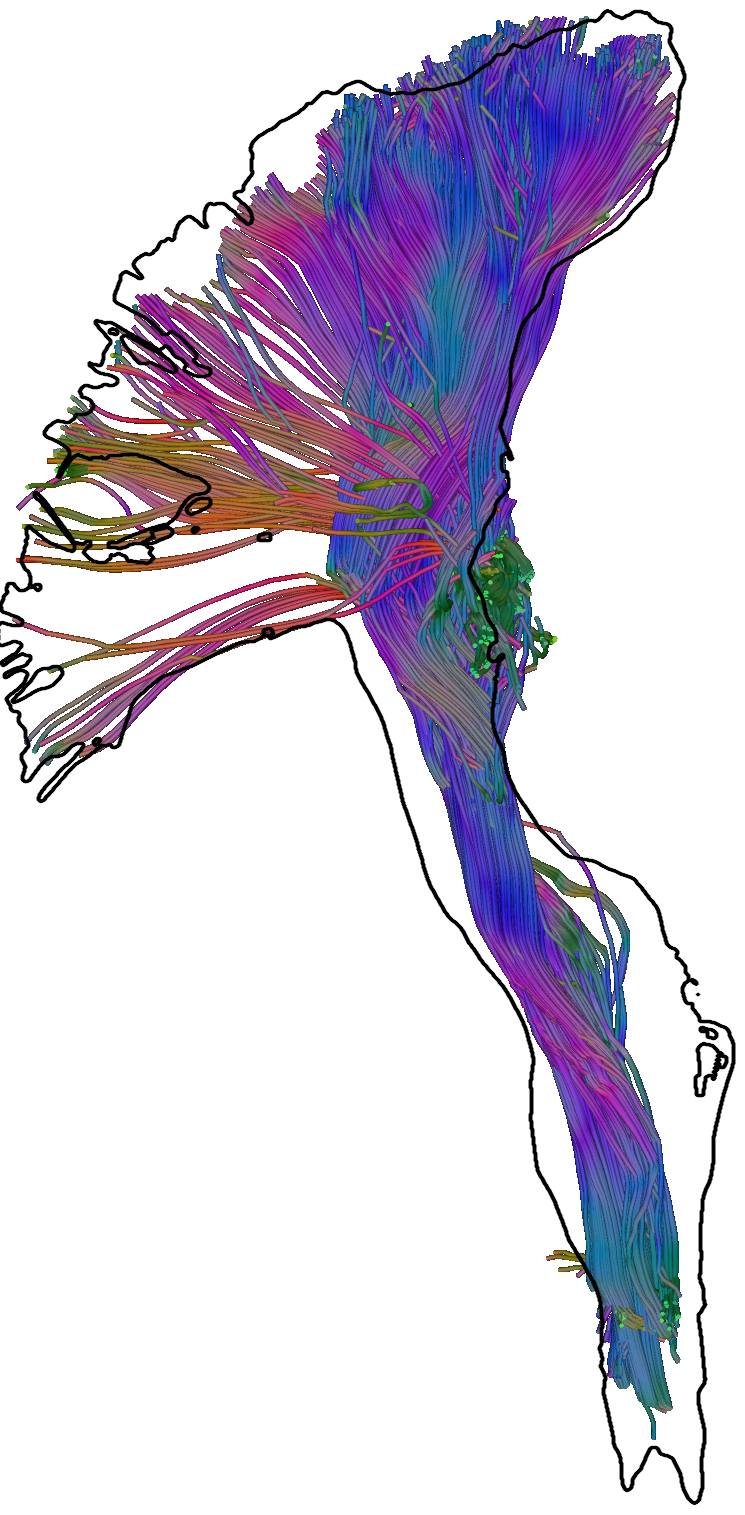
\includegraphics[width=\linewidth]{cst-sel-c}
		\caption{Selection model}
	\end{subfigure}
	\begin{subfigure}[b]{0.45\linewidth}
		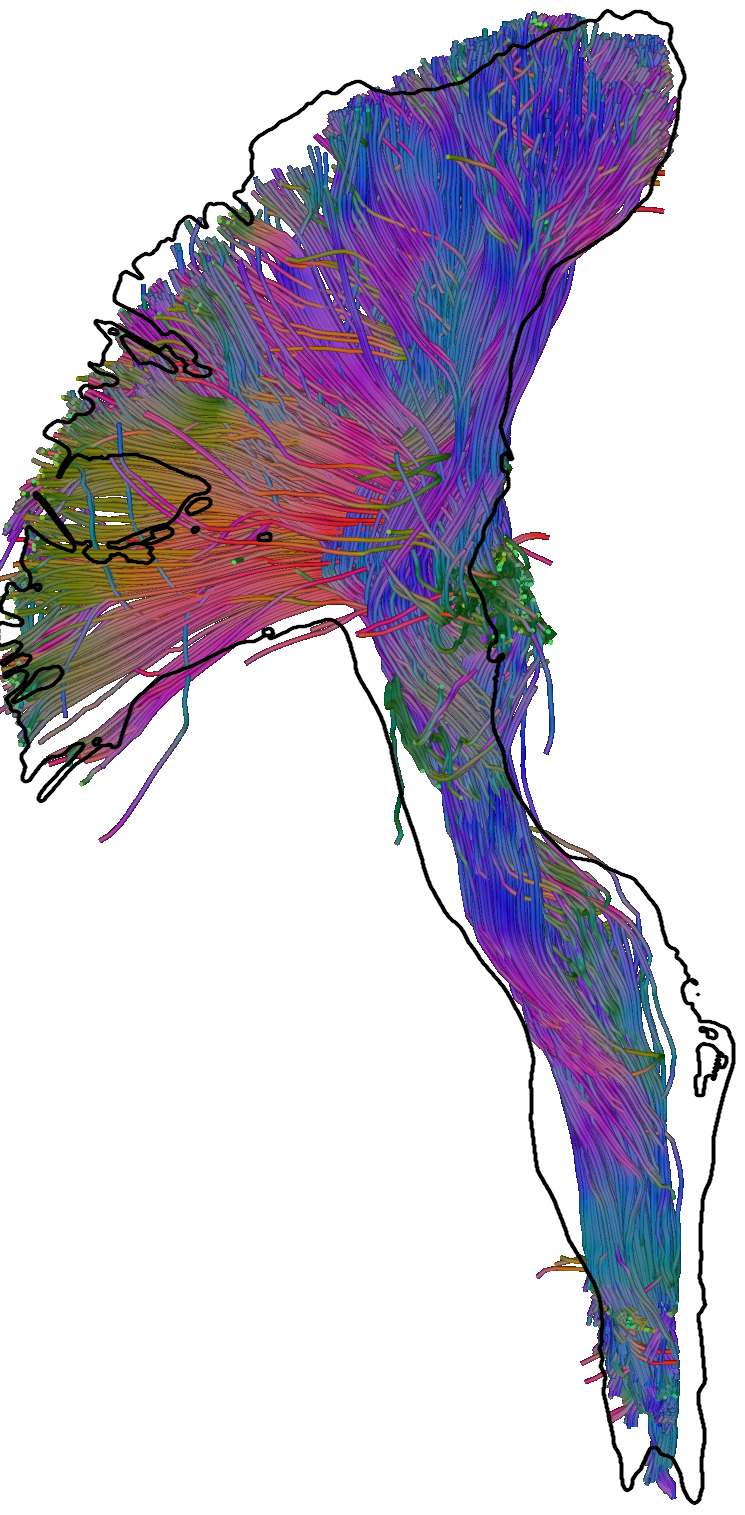
\includegraphics[width=\linewidth]{cst-sel-bootstrap-c}
		\caption{Consensus Selection Model}
\end{subfigure} \\
\caption{Reconstruction of the right Corticospinal Tract. The reference
tractography is set as grey background and the reconstruction as XYZ colored
foreground to make comparison more intuitive. The seed region is indicated by
the black dashed line. }
	\label{fig:CST}
\end{figure}
As a first experiment we tract the right Cortiscospinal Tract (CST) from a seed
region, which is indicated with a dashed black line in Fig. \ref{fig:CST}. This tract is
known for its huge lateral spread, which is difficult to recover. The
novel proposed consensus approach increases the completeness of the lateral
spread especially for the selection model dramatically. While the selection
model is only able to recover a few single streamlines within this area the
consensus approach improves this area significantly. The consensus model also
improves the average and low-rank model. Here the spread is present in the base
model, but get denser by applying the consensus model. Further the streamlines
seems to be more aligned.

\begin{figure*}[h]
	\centering
	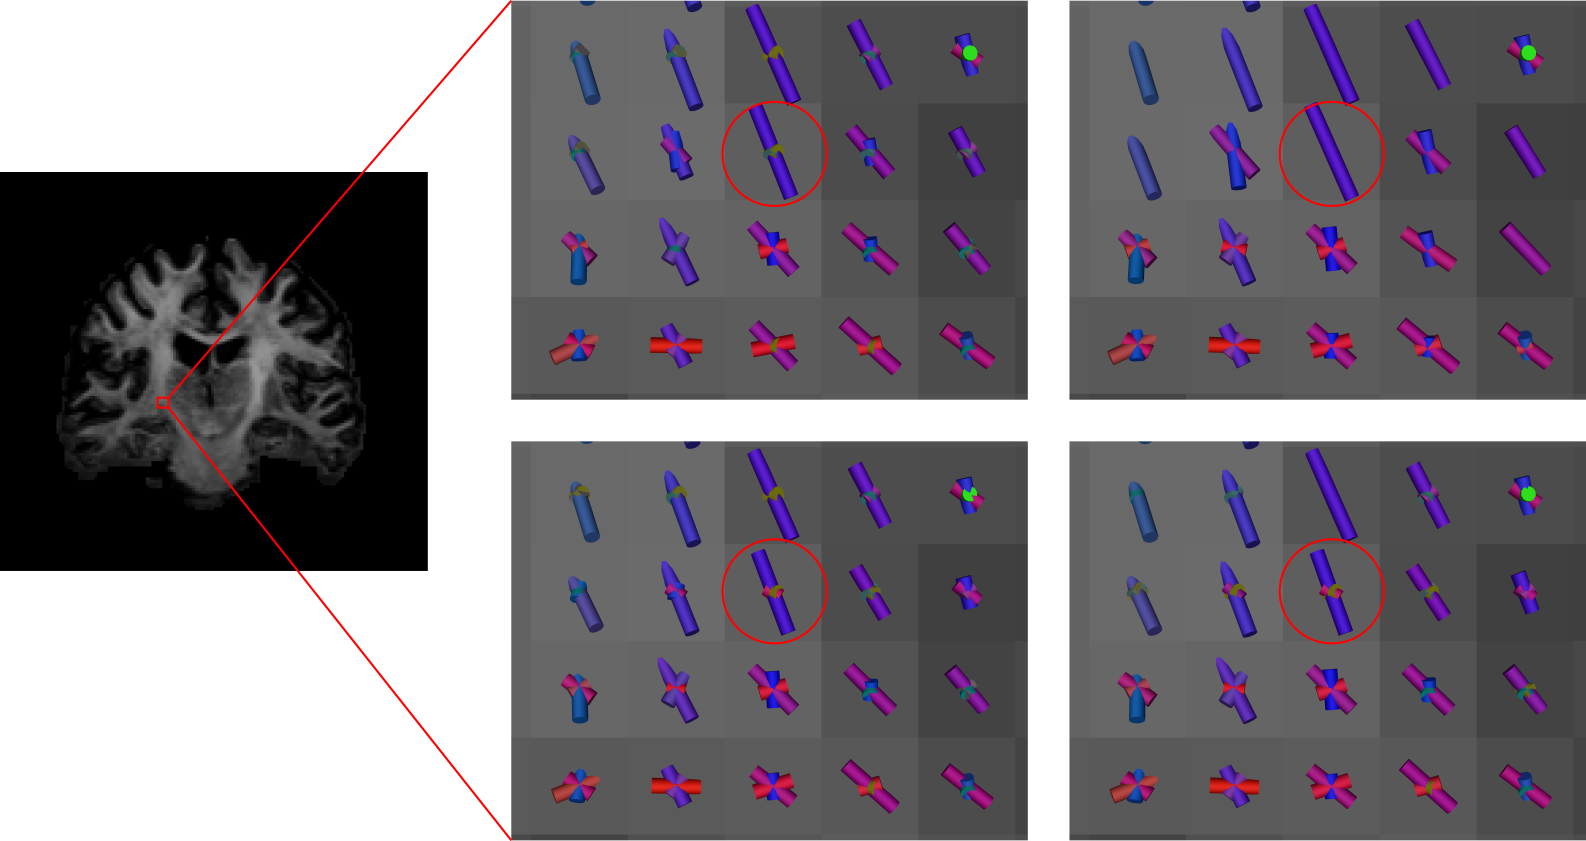
\includegraphics[width=\linewidth]{dir}
	\caption{Reconstructed fiber orientations of the different models, the
	red box in the left image denotes the position within the brain. Top row
shows models without consensus bootstrapping, bottom row with consensus
bootstrapping. Left: Averaging model. Right: selection model.}
	\label{fig:directions}
\end{figure*}

This observation can be further explained by inspecting the multi vector fields
on Fig. \ref{fig:directions}. The most obvious difference between the average and
selection model is, that the average model has three fibers in
each voxel, while the selection model contains often just one fiber in a voxel.
For the tracking approach this leads to much more spread as seen in the
reconstruction of the CST. However, this also leads to much more 'fuzziness'
within the average model reconstruction. 
Applying the consensus to the average
and selection model leads to quiet similar multi vector fields as it can be seen
in the red circle. Within this voxel the average and selection model are
dissimilar but the consensus model agrees. This is also the case for the most
other voxels. However, in some voxels we see differences, as for example in the
voxel on top of the red circle where the average model contains $2$ fibers,
while the selection model contains just one fiber. Therefore, we conclude that
the consensus selection model and the average model are very similar, which is a
reason for the great improvement of the consensus selection model. 

\subsection{Quantitative Comparison}
\begin{figure}[t]
	\centering
	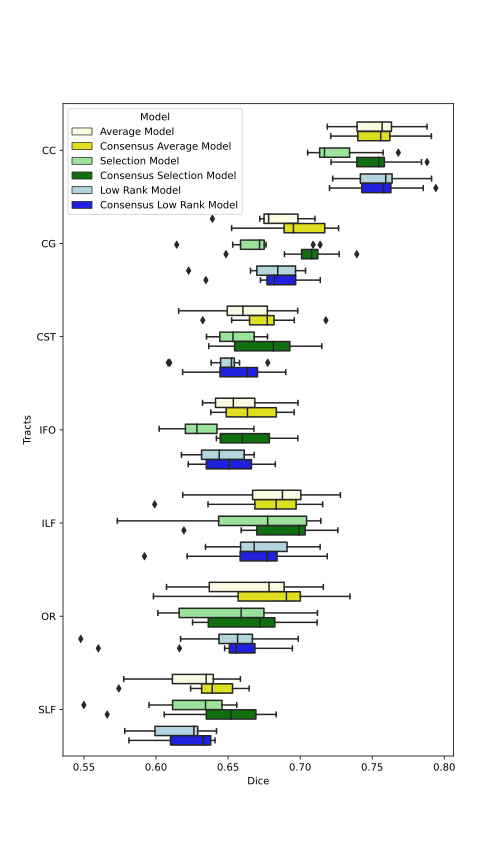
\includegraphics[width=\linewidth]{comparison-dice}
	\caption{Boxplots of the dice scores of all patients for all models. All
	subtracts are preprocessed seperatly, then merhed and the dice scores
are calculated for a binary mask of the joint subtracts.}
	\label{fig:Dice}
\end{figure}

\begin{table*}
\centering
\begin{tabular}{p{4cm}p{1.5cm}p{1cm}p{1cm}p{1cm}p{1cm}}
	{}  & \rot{Consensus   Average  Model} & \rot{Selection Model} &
	\rot{Consensus Selection Model} & \rot{Low Rank Model} & \rot{Consensus
	Low Rank Model} \\ \hline  
Average Model &   {\cellcolor{lightgreen} 0.001} & {\cellcolor{lightred} 0.001}
& {\cellcolor{lightgreen} 0.002} & {\cellcolor{lightred} 0.001} & 0.063 \\
Consensus Average Model &   & {\cellcolor{lightred} 0.001} & 0.900 &
{\cellcolor{lightred} 0.001} & {\cellcolor{lightred} 0.001} \\
Selection Model &    & & {\cellcolor{lightgreen} 0.001} & 0.900 & 0.494 \\
Consensus Selection Model &  &  &  & {\cellcolor{lightred} 0.001} &
{\cellcolor{lightred} 0.001} \\
Low Rank Model &   &
 &   & & 0.494 \\
\end{tabular}
\caption{Comparison of different models by Nemenyi post-hoc test. All $p$ values
below $0.05$ are marked. If the top model is significantly better in green else
in red.}
	\label{tab:sig}
\end{table*}


For a representative experiment we have reconstructed the corpus callosum (CC), the
cingulum (CG), the coricospinal tract (CST), the inferior fronto-occipital (IFO)
and the inferior longitudinal fasciculus (ILF), the optic radiation (OR), and
the superior longitudinal fasciculus (SLF). In the reference tragtographies, the
CC and SLF tracts were divided into subtracts, which we have merged into a single
tract. Further, we have merged the left and right parts of each tract. We have
evaluated the reconstruction quality by Dice score which is defined as
\[ 
	DICE = \frac{2 |RD \cap TR |}{|TR| + |RD|} ,
\]
where $RD$ denotes the reference data and $TR$ the tracking results
\cite{SCHILLING2019194}. A high Dice score is desired, as it denotes a high
overlap and a low overreach. To validate the results further, we applied a
Friedman test on model level to investigate if a model is significantly better
than any other model \cite{doi:10.1080/01621459.1937.10503522}. Post-hoc we
applied Nemenyi test to identify which models are significantly different
\cite{Nemenyi}.  


Figure \ref{fig:Dice} and Table \ref{tab:sig} summarize the results of our
quantitative comparison. In Fig. \ref{fig:Dice}, results from the average,
selection and low-rank model with and without use of the consensus model are
visualized using box plots to show the tract wise distribution of the Dice
scores. In Table \ref{tab:sig} the results of the post hoc Nemenyi tests are
shown. As a first result we denote that the Friedman test has shown that there
are significant differences between the models. 

To justify our previous work further, we are interested in the comparison of the
average, selection and low-rank model. The first impression from Fig.
\ref{fig:Dice} is that the average model is preferable to the other models and
that it depends on the tract if we prefer the selection or the low-rank model.
As it is visible in Table \ref{tab:sig} the improvement of the average model to
the other models is significant, while neither the selection model nor the
low-rank model is preferable to
the other. Therefore, we conclude that the average model, which we have proposed
within our last paper is significantly better than both other models. 

Within this work, we are more interested in the consensus model. Therefore, we
investigate if the improvement is significant between the model with and without
the application of the consensus. From Fig. \ref{fig:Dice} we can conclude, that
in 6 out of 7 tracts the consensus average model has an higher average Dice
score than the average model, that the consensus selection model has always an
higher Dice score, and that the consensus low-rank model has in 4 out of 7
tracts an higher Dice score. These changes are significant for the average and
selection model, while they are not significant for the low-rank model. 

Further, we want to compare the consensus models against each other. From Fig
\ref{fig:Dice} it seems that the consensus average and selection model are
preferable compared to the consensus low-rank model. Both models are equally
good compared by the mean dice score. This gets justified by the significance
tests. The consensus average as well as the consensus selection model are
significantly better than the consensus low-rank model. 

Overall we have shown that the consensus model improves our previously proposed
models significantly. However, the improvement by average Dice score is only for
the selection model large. 
\subsection{Computational Effort}
All experiments were computed on an Intel i9 with 3.3 GHz and 64 GB RAM. The
following durations are denoted in h:min:s or min:s.

The computation of a single bootstrap data sample took 1:10 on a single core,
multi-threaded fourth order fODF estimation took 4:33, the computation of the
selection model took 1:10, the computation of the averaging model took 1:30 and
the computation of the rank-3 model 0:40. The calculation of 100 bootstraps took
therefore 8:08:00, using all threads to create the bootstrap data as well as the
models. This also includes the computation of the consensus model, which on its
own took 11:00. The tracking itself is independent of the preprocessing steps.
It took approximately 3:30 for a bundle such it is shown in Figure
\ref{fig:Dice} on a single thread including postprocessing.  



\section{Conclusion}
\label{sec:conclusion}
In this work, we presented and evaluated two approaches to reduce different types of uncertainty in diffusion MRI tractography. The first one, model averaging, relies on Bayesian model comparison, and reduces the model uncertainty in crossing fiber tractography that results from having to select the most suitable number of fibers in each tracking step. The second one, bootstrap consensus, primarily aims to reduce data uncertainty, but we observe that it also reduces model uncertainty due to an interdependency of both. In either case, we fuse information from multiple fiber estimates to obtain a more reliable basis for fiber tractography.

Our experimental results demonstrate that each of the two approaches by itself makes dMRI tractography more accurate, as confirmed both by qualitative results and a formal statistical analysis. Even though combining both methods yielded an additional benefit, in terms of practical utility, it is worth keeping in mind that the additional computational expense from model averaging is marginal (in our experiments, it added 20 seconds to the pre-processing), while the computational effort for bootstrapping is substantial (in our experiments, more than eight hours per dataset).

We expect that, in many use cases, this will make model averaging the more pragmatic choice. Despite this, bootstrapping also provided further insights, most importantly, on the interaction between data and model uncertainty, and the effect of model averaging on the uncertainty in fiber direction estimates.

\section*{Acknowledgments}

We thank Gemma van der Voort (University of Bonn) for her initial proof-of-concept implementation of tractography with model averaging, and for providing feedback on our manuscript. This work was funded by the Deutsche Forschungsgemeinschaft (DFG, German Research Foundation) -- 422414649.
Data were provided by the Human Connectome Project, WU-Minn Consortium (Principal Investigators: David Van Essen and Kamil Ugurbil; 1U54MH091657) funded by the 16 NIH Institutes and Centers that support the NIH Blueprint
for Neuroscience Research; and by the McDonnell Center for Systems Neuroscience at Washington University.

%%% Local Variables:
%%% mode: latex
%%% TeX-master: "../main"
%%% End:

\printbibliography
\end{document}
